%--------------------------- Hoda Abbasi ----------------------------
%----------------------- 16 March 2016 ------------------------

\documentclass[]{book}
\input Latex_macros/Definitionen.tex
\usepackage{a4}
\usepackage{graphicx}
\usepackage{tikz-qtree}
\usepackage{latexsym}
\usepackage{amssymb}
\usepackage{tikz}
\usetikzlibrary{arrows}
\setcounter{tocdepth}{4}
\setcounter{secnumdepth}{4}
\usepackage{enumerate}
\usepackage[active]{srcltx}
\usepackage[all]{xy}
%\usepackage{xspace}
%\usepackage{multicol}
%\usepackage{multirow}
%\usepackage{caption}
%\usepackage{Latex_styles/slashbox}
%\usepackage{bussproofs}
%\usepackage{xr}
\usepackage{todonotes}
\usepackage{etex}
\usepackage{mathtools} % For \mathmakebox
\newcommand{\Schrift}{report}
   

%%%%%%%%%%%%%%%%%%%%%%%%%%% Symbols %%%%%%%%%%%%%%%%%%%%%%%%%%%%%%%%%%%%%
\DMO{\dhardness}{dys}
\DMO{\nwid}{nwid}

\DMO{\twidth}{tw}
%--------------------------------------------------------------------------------------------------------------------------------------
\begin{document}
\title{Hardness measures of clause-sets}

\author{Hoda Abbasi\\
             PhD Candidate\\
             Computer Science Department\\
             Swansea University\\}
\maketitle
%--------------------------------------------------------------------------------------------------------------------------------------
\tableofcontents

%***************************************************************************************************************************************
%***************************************************************************************************************************************************************
\chapter{Introduction}
\label{cha:Introduction}

???????????

The aim of this report is to investigate different hardness measures for a clause-set in the literature and then, 
to propose a method based on Prover-Delayer games. 

The report is organized as follows. In Chapter \ref{cha:Preliminaries} some general preliminaries are presented.
Then, in Chapter \ref{cha:Hardness Measures} hardness is defined as a measure for complexity of unsatisfiable clause-set.
This measure, then is extended for arbitrary clause-set. 
Chapter \ref{cha:XOR-constraints} explains a system of XOR-constraint and ??????

In Chapter \ref{cha:hdgame}, the proposed method to obtain the hardness of a clause-set is given.
Finally, Chapter \ref{cha:concl} presents some questions regarding hardness measures and the hardness game and then, it concludes the report.
%***************************************************************************************************************************************
%***************************************************************************************************************************************************************
\chapter{Preliminaries}
\label{cha:Preliminaries}

\section{Variables}
\label{sec:Variables}

\begin{defi}\label{def:var}
      The set of ``variables'' is denoted by \bmm{\Va}. For every variable $v \in \Va$ its \textbf{domain} is a finite and non-empty set, denoted by 
	  $\bmm{D_v} \ne \es$. Together $(\Va, (D_v)_{v \in \Va})$ is the \textbf{variable-frame}.
      \begin{itemize}
            \item A \textbf{standard domain} is of the form $D_v = \tb 0m \subset \NNZ$ for some $m \in \NNZ$.
            \item A \textbf{boolean variable} $v$ has domain $D_v = \set{0,1}$.
            \item The domain-size of variables is denoted by $\bmm{\dos}: \Va \ra \NN$, with $\dos(v) := \abs{D_v}$.
      \end{itemize}
      It is assumed that for every occurring domain-size $m \in \dos(\Va)$ there are infinitely many variables with this domain-size, that is, $\dos^{-1}(m)$ is infinite.
      \begin{itemize}
            \item The \textbf{standard boolean var-set} is $\Va := \NN$, where all variables are boolean.
            \item The \textbf{standard non-boolean var-set} is $\Va := \NN \times \NN_{\ge2}$, where all variables have a standardised domain, and where 
			$\dos((n,m)) = m$ for $(n,m) \in \Va$.
      \end{itemize}
\end{defi}
Remarks:
\begin{enumerate}
      \item For variables $v$ with standard domains holds $D_v = \tb{0}{\dos(v)-1}$.
      \item It seems not useful to allow domain-size zero; such variables couldn't be assigned at all.
      \item Typically we just mention $\Va$ in the basic set-up, not the full variable-frame $(\Va,
      D_v)_{v \in \Va})$, which is understood implicitly. Then one says whether we have only boolean variables or also non-boolean variables.
\end{enumerate}

\begin{examp}\label{exp:var}
      The standard boolean variables are $1, 2, 3, \dots \in \NN$, the standardd non-boolean boolean variables(!) are $(1,2), (2,2), (3,2), \dots \in \NN \times \set{2}$. 
	  The standard ternary variables (three-valued) are $(1,3), (2,3), (3,3), \dots \in \NN \times \set{3}$.
\end{examp}
%--------------------------------------------------------------------------------------------------------------------------------------
\section{Partial assignments}
\label{sec:Partialassignments}

\begin{defi}\label{def:Pass}
      A \textbf{partial assignment} is a map $\vp$ with domain $\bmm{\var(\vp)} := \dom(\vp) \in \pote(\Va)$, such that for all $v \in \var(\vp)$ holds $\vp(v) \in D_v$. 
	  The set of all partial assignments is denoted by \bmm{\Pass}.

      For $V \in \pote(\Va)$ let $\bmm{\Tass(V)} := \set{\vp \in \Pass : \var(\vp) = V}$ be the set of \textbf{total assignments} over $V$.

      A special partial assignment is $\bmm{\epa} := \es \in \Pass$ (the \textbf{empty partial assignment}).
\end{defi}
Remarks:
\begin{enumerate}
      \item For variables $v_1, \ldots, v_n \in \Va, \; n\in \mathbb{N}_0$ with $v_i \neq v_j$ for $i\neq j$, and truth values $\varepsilon_1, \ldots, \varepsilon_n \in \{0,1\}$ we write
      \begin{displaymath}
            \pmb{\langle v_1 \to \varepsilon_1, \ldots, v_n \to \varepsilon_n\rangle}
      \end{displaymath}
      for the partial assignment with
      \begin{displaymath}
            \mbox{domain} \; \{v_1, \ldots, v_n\}
      \end{displaymath}
      which maps $v_i \mapsto \varepsilon_i$.
      \item So $\Tass(V) = \prod_{v \in V} D_v$.
      \item $n(\varphi) := \abs {\var(\varphi) }$ (the number of variables in a partial assignment).
\end{enumerate}

%--------------------------------------------------------------------------------------------------------------------------------------
\section{Literals}
\label{sec:Litsvar}

\begin{defi}\label{def:litdervar}
      For a variable-frame $(\Va, (D_v)_{v \in \Va})$, a \textbf{literal} is a pair $(v,\ve)$ with $v \in \Va$ and $\ve \in D_v$. The set of all literals is denoted by 
	  $\bmm{\Lit}$. In other words, the set $\Lit$ of \textbf{literals} (over $\Va$) is defined as:
      $$\Lit( \Va): = \Va \times \{0,1\}.$$
      For $(v,\ve) \in \Lit$:
      \begin{enumerate}
            \item $\bmm{\var((v,\ve))} := \proj_1((v,\ve)) = v \in \Va$.
            \item $\bmm{\val((v,\ve))} := \proj_2((v,\ve)) = \ve$.
            \item \textbf{positive} in case of $\varepsilon = 0$.
            \item \textbf{negative} in case of $\varepsilon = 1$.
      \end{enumerate}
      Literals $x, y \in \Lit$ \textbf{clash} (or ``have a conflict'') if $\var(x) = \var(y)$ and $\val(x) \ne \val(y)$. For $L \sse \Lit$ we say that 
	  \textbf{$L$ is clash-free} if there are no $x, y \in L$ which clash.
\end{defi}
Remarks:
\begin{enumerate}
      \item As customary, in case we are not especially interested in the underlying set   $\Va$ of variables, we will just use  $\Lit$ instead of $\Lit$($\Va$)
      \item The set of partial assignments is the set of clash-free $\vp \in \pote(\Lit)$.
      \item Simple properties:
      \begin{enumerate}
            \item $({}^{\overline{~~}}): \Lit \to  \Lit.$
            \item $\overline{(v, \varepsilon)}: = (v, 1-\varepsilon).$
            \item For a literal $x$ we call $\overline{{\bm x}}$ the \textbf{complement} of $x$ and we have
            $$\forall x \in \Lit: \overline{\overline{x}} = x.$$
      \end{enumerate}
\end{enumerate}
\begin{examp}\label{}
      Consider a variables $a\in  \Va$. Using the identification of variables and positive literals, we have
      \begin{eqnarray*}
            &a = (a,0)& \\
            &\overline{a} = \overline{(a,0)} = (a,1)&\\
            &\overline{\overline{a}} = \overline{(a,1)} = (a,0) = a&\\
            &\var(a) = \var((a,0)) = a& \\
            &\var(\overline{a}) = \var((a,1)) = a. &
      \end{eqnarray*}
\end{examp}
%--------------------------------------------------------------------------------------------------------------------------------------
\section{Clauses}
\label{sec:Clauses}

\begin{defi}\label{def:clauses}
      For a set $L \sse \Lit$ we define:
      \begin{itemize}
            \item $\bmm{\var(L)} := \set{\var(x) : x \in L}$
            \item $\bmm{\lit(L)} := \set{x \in \Lit : \var(x) \in \var(L)}$
            \item $\bmm{\ol{L}} := \lit(L) \sm L$.
      \end{itemize}
\end{defi}
Remarks:
\begin{enumerate}
      \item So $\var(L)$ is the set of ``variables of $L$'', $\lit(L)$ is the set of ``literals having a variable in $L$'', while $\ol{L}$ 
	  is the set-complement of $L$ in the set of literals with variables in $L$.
      \item For $\vp \in \Pass$ holds $\ol{\vp} \in \Pass$ iff $\dos(\vp) \sse \set{1,2}$.
      \item $\set{\lit(\set{x})}_{x \in \Lit}$ is a partition of $\Lit$, and the partial assignments are the finite sets of literals which 
	  intersect with each element of this set-system in at most one element.
      \item For a finite $L \subset \Lit$ the following properties are equivalent:
      \begin{enumerate}
            \item $L$ is clashfree.
            \item $\fa\, x \in \Lit : \abs{\lit(\set{x}) \cap L} \le 1$.
            \item $\abs{L} = \abs{\var(L)}$.
      \end{enumerate}
      \item If $L$ is a set of boolean variables, then $\lit(L) = L \cup \ol{L}$.
      \item If $L$ is a set of non-boolean variables, then $\ol{L} = \emptyset$.
\end{enumerate}
\begin{examp}\label{exp:lit1}
      For sets $L_1, L_2 \sse \Lit$ with boolean variables, if $L_1 = \{1, 2, 3 \}$ and $L_2 = \{1, -1, -2, 3 \}$ we have:
      $$lit(L_1) = \{1, -1, 2, -2, 3, -3\}$$
      $$lit(L_2) = \{1, -1, 2, -2, 3, -3\}$$
\end{examp}
\begin{examp}\label{exp:lit1}
      For sets $L_1, L_2 \sse \Lit$ with non-boolean variables, if $L_1 = \{1, 2, 3 \}$, and $L_2 = \{1, -1, -2, 3 \}$ we have:
      $$lit(L_1) = \{1, 2, 3\}$$
      $$lit(L_2) = \{1, -1, -2, 3\}$$
\end{examp}
\begin{defi}\label{def:cl}
      A \textbf{clause} is a finite and clash-free set of literals, the set of all clauses is denoted by
      $$\bmm{\Cl} := \set{C \in \pote(\Lit) : \abs{C} = \abs{\var(C)}}.$$
      A special clause is $\bmm{\bot} := \es \in \Cl$, the \textbf{empty clause}.
\end{defi}
\begin{lem}\label{lem::CLPASS}
      $\Cl = \Pass$.
\end{lem}
Remarks:
\begin{enumerate}
      \item Since a clause is a \textit{set}, every element occurs only once in a clause;
      \item There is no order on the elements of a clause.
      \item So to partial assignments $\vp \in \Pass$ we can apply the operations which can be applied to sets of literals. Especially
      $$\ol{\vp} = \set{(v,\ve) \in \Lit : v \in \var(\vp) \wedge \vp(v) \ne \ve}.$$
\end{enumerate}
%--------------------------------------------------------------------------------------------------------------------------------------
\section{Clause-sets}
\label{sec:cls}

\begin{defi}\label{def:cls}
      A \textbf{clause-set} is a finite set of clauses, the set of all clause-sets is denoted by $\bmm{\Cls} := \pote(\Cl)$.

      A special clause-set is $\bmm{\top} := \es \in \Cls$, the \textbf{empty clause-set}.
\end{defi}
\begin{defi}\label{def:cls2}
      The clause-set $F \in \Cls$ where each clause contains at most $k$ literals (has width at most $k$) is called \textbf{k-}$\Cls$.
      This means that $\abs {C} \le k$ \cite{h5}.
\end{defi}
\begin{defi}\label{def:cls3}
      A literal $x$ is called \textbf{pure} for $F$ if \ $\overline{x} \not \in \bigcup F$ 
      (the literals occuring in $F$ are give by $\bigcup F \subset \Lit$) \cite{h5}.
\end{defi}
\begin{defi}\label{def:cls4}
      For $F \in \Cls$:
      \begin{enumerate}
            \item $\bmm{\var(F)} := \bc_{C \in F} \var(C) \in \pote(\Va)$.
            \item $\bmm{\lit(F)} := \lit(\var(F)) \in \pote(\Lit)$ or $\lit(F) := \var(F) \cup \overline{\var(F)}$.
            \item $\bmm{n(F)} := \abs{\var(F)} \in \NNZ$ (the number of variables).
            \item $\bmm{c(F)} := \abs{F} \in \NNZ$ (the number of clauses).
            \item $\bmm{\ell(F)} := \sum_{C \in F} \abs{C} \in \NNZ$ (the number of literal occurrences).
      \end{enumerate}
\end{defi}
\begin{examp}\label{exp:classescls}
  $\Cls_{n=0} = \Cls_{\ell=0} = \set{\top, \set{\bot}}$, $\Cls_{c=0} = \set{\top}$, and $\Cls_{n<0} = \es$ \cite{h9}.
\end{examp}
\begin{defi}\label{def:cls6}
      Clause-sets $F,G$ are called \textbf{isomorphic}, if the variables of $F$ can be renamed and potentially flipped so that $F$ is 
	  turned into $G$. More precisely, an isomorphism $\alpha$ from $F$ to $G$ is a bijection $\alpha : \lit(F) \rightarrow \lit(G)$ 
	  which preservers complementation $(\alpha(\ol x) = \overline {\alpha(x)}$, and which maps the clauses of $F$ precisely to the 
	  clauses of $G$; when considering multi-clause-sets, then the isomorphism must preserve the multiplicity of clauses (that is, 
	  $G(\alpha(C)) = F(C)$ for all $C \in \Cl$) \cite{h9}.
\end{defi}
Remarks:
\begin{enumerate}
      \item No clause may occur more than once in a clause-set.
      \item There is no order on the elements of a clause-set.
\end{enumerate}
\begin{examp}\label{exp:cls}
      Some examples of clause-sets are as folow:
      $$\left\{\{a\}, \{\overline{a}\}\right\}$$
      $$\left\{\{a,b\}, \{\overline{a},b\}, \{a, \overline{b}\}, \{\overline{a},\overline{b}\}\right\}$$
      $$\left\{\{a\}, \{\overline{a},b\}, \{\overline{a}, \overline{b}, c\}, \{\overline{a}, \overline{b}, \overline{c}\}\right\}$$
\end{examp}
%%%%%%%%%%%%
\begin{defi}\label{def:fullcls}
      A clause $C$  for a clause-set $F$ is called \textbf{full} if $C \in F$ and $\var(C) = \var(F)$, while a clause-set 
	  $F$ is called full if every clause is full. For a finite set $V$ of variables let
      \begin{displaymath}
      \bmm{A(V)} := \set{C \in \Cl : \var(C) = V} \in \Cls.
      \end{displaymath}
      Obviously $A(V) \in \Clash$ is the set of all $2^{\abs{V}}$ full clauses over $V$, and $F \in \Cls$ is full iff 
	  $F \sse A(\var(F))$. We use $\bmm{A_n} := A(\tb 1n)$ for $n \in \NNZ$. Dually, a variable $v \in \Va$ is called 
	  \textbf{full} for a clause-set $F$ if for all $C \in F$ holds $v \in \var(C)$. A clause-set is full iff every 
	  $v \in \var(F)$ is full \cite{h9}.
\end{defi}

\begin{examp}\label{exp:An}
  In general $n(A_n) = n$, $c(A_n) = 2^n$ and $\delta(A_n) = 2^n-n$. Initial cases are $A_0 = \set{\bot}$, $A_1 = \set{\set{1},\set{-1}}$ 
  and $A_2 = \set{\set{-1,-2},\set{-1,2},\set{1,-2},\set{1,2}}$ \cite{h12}.
\end{examp}

\begin{examp}\label{exp:measurecls}
  For $F := \set{\bot, \set{1},\set{-1,2}}$ we have:
  \begin{enumerate}
  \item $\var(F) = \{1, 2\},\ \lit(F) = \{- 1, 1,- 2, 2\},\ \bigcup F = \{-1, 1, 2\}$.
  \item Literal 2 is pure for $F$ (the other literals in $\lit(F)$ are not pure).
  \item $n(F) = 2$, $c(F) = 3$, $\delta(F) = 1$, $\ell(F) = 3$.
  \item $\set{-1,2}$ is a full clause of $F$, while the two other clauses are not full.
  \item $F$ has no full variable, while $F \sm \set{\bot}$ has the (single) full variable $1$.
  \end{enumerate}
  The standard ``complete'' full clause-sets are $A_0 = \set{\bot}$, $A_1 = \set{\set{-1},\set{1}}$,
  \begin{displaymath}
    A_2 = \set{\set{-1,-2},\set{-1,2},\set{1,-2},\set{1,2}},
  \end{displaymath}
  and so on \cite{h12}.
\end{examp}
%--------------------------------------------------------------------------------------------------------------------------------------
\section{The operation of partial assignments on clause-sets}
\label{sec:oppasscls}

\begin{defi}\label{def:oppassCls}
      For $\vp \in \Pass$ and $F \in \Cls$:
      $$\bmm{\vp * F} := \set{C \sm \vp : C \in F \wedge C \cap \ol{\vp} = \es} \in \Cls.$$
\end{defi}
Remarks:
\begin{enumerate}
      \item Simple properties:
      \begin{enumerate}
            \item $\vp * (F \cup G) = \vp * F \cup \vp * G$.
            \item $\vp * \set{C} = \set{\bot}$ iff $C \sse \vp$.
            \item $\vp * \set{C} = \top$ iff $C \cap \ol{\vp} \ne \es$.
            \item $\vp = \set{x \in \Lit : \vp * \set{x} = \set{\bot}}$.
            \item $\vp * F = \top \Lra \fa\, C \in F : C \cap \ol{\vp} \ne \es$.
            \item $\bot \in \vp * F \Lra \ex\, C \in F : C \sse \vp$.
            \item $\bot \in F \Ra \bot \in \vp * F$.
            \item $\vp * \top = \top$.
            \item $ var(\vp * F) = F \Leftrightarrow var(\vp) \cap var(F) = \emptyset$.
            \item $ var(\vp * F) \subseteq var(F) \setminus var(\vp)$.
      \end{enumerate}
      \item If $\vp * F \in \set{\top, \set{\bot}}$ and $\vp' \supseteq \vp$, then $\vp' * F = \vp * F$.
      \item More generally, for $\vp' \supseteq \vp$ with $(\var(\vp') \sm \var(\vp)) \cap \var(\vp * F) = \es$ holds $\vp' * F = \vp * F$. 
	  Especially for $\var(\vp) \cap \var(F) = \es$ holds $\vp * F = F$.
\end{enumerate}

\begin{examp}\label{exp:op1}
      Some examples of operation of partial assignments are as folow:
      $$\varphi_{\{a,\overline{b},c\}} = \langle a, \overline{b}, c\to 0\rangle = \langle a\to 0, b\to 1, c\to 0 \rangle $$
      $$C_{\langle x\to 0, y\to 1, z\to 0 \rangle} = \{x, \overline{y}, z\}$$
      $$\langle a\to 1 \rangle * \left\{\{a,b,c\}, \{\overline{a}, \overline{c}\}, \{\overline{b}, \overline{c}\} \right\} = \left\{\{\overline{c}\}, \{\overline{b}, c\} \right\}$$
      $$\langle a\to 0, b\to 1, c\to 0 \rangle * \left\{\{a,b,x\}, \{a,\overline{b},c\}, \{\overline{x}, \overline{y}\}, \{a,c,x\} \right\} = \left\{\bot, \{\overline{x}, \overline{y}\}, \{x\}\right\}$$
      (a falsifying assignment)
      $$\langle x\to 1, y\to 0, z\to 1 \rangle * \left\{\{x,y,\overline{z}\}, \{x,\overline{y},z\}, \{\overline{x}, \overline{y}\}, \{x,y\} \right\} = \top$$
      (a satisfying assignment)
\end{examp}
%--------------------------------------------------------------------------------------------------------------------------------------
\section{Composition of partial assignments}
\label{sec:Compositionpass}

\begin{defi}\label{def:comppass}
      For $\vp, \psi \in \Pass$: $\bmm{\vp \circ \psi} := \psi \cup (\vp \sm \lit(\psi)) \in \Pass$.
      In other words: For the composition of two partial assignments take their ``union'' for non-conflicting variables, while in case of a 
	  conflict the right assignments ``wins''.
\end{defi}
\begin{lem}\label{lem:passmon}
      $(\Pass,\circ,\epa)$ is a monoid (an associative groupoid with identity element). It is generated by 
      the \textbf{elementary partial assignments} $\langle v\to \varepsilon\rangle$ for $v\in \Va$ and $\varepsilon \in \{0,1\}$, and the ``defining relations'' are
      $$\langle v\to \varepsilon \rangle \circ \langle v\to \varepsilon' \rangle = \langle v\to \varepsilon' \rangle $$
      $$\langle v\to \varepsilon \rangle \circ \langle w\to \varepsilon' \rangle = \langle w\to \varepsilon' \rangle \circ \langle v\to \varepsilon \rangle$$
      for $v, w\in \Va, v\neq w$, and $\varepsilon, \varepsilon' \in \{0, 1\}$.
\end{lem}

Remarks:
\begin{enumerate}
      \item Simple properties:
      \begin{enumerate}
            \item $\var(\varphi \circ \psi)  = \var(\varphi)\cup \var(\psi)$.
            \item $\varphi \circ \emptyset  = \emptyset \circ \varphi = \varphi$.
            \item $\varphi \circ (\psi \circ \vartheta) = (\varphi \circ \psi) \circ \vartheta$.
      \end{enumerate}
\end{enumerate}
\begin{lem}\label{lem:comcomp}
  For $\vp, \psi \in \Pass$ the following properties are equivalent:
  \begin{enumerate}
  \item $\vp \circ \psi = \psi \circ \vp$.
  \item $\vp \cup \psi \in \Pass$.
  \item $\vp, \psi$ do not clash, that is, $\vp \cap \ol{\psi} = \es$.
  \end{enumerate}
\end{lem}
\begin{examp}\label{exp:cmp}
      Consider variables $a,b,c,d \in \Va$. By the term $\langle a\to 0, b\to 1 \rangle$ the partial assignment $\varphi$ with domain 
	  $\var(\varphi) = \{a, b\}$ and $\varphi(a) = 0$ and $\varphi(b) = 1$ is denoted.
      Examples for the defining relations are:
      $$\langle a\to 0 \rangle \circ \langle a\to 1 \rangle = \langle a\to 1 \rangle $$
      $$\langle b\to 1 \rangle \circ \langle b\to 1 \rangle = \langle b\to 1 \rangle $$
      $$\langle c\to 1 \rangle \circ \langle c\to 0 \rangle = \langle c\to 0 \rangle$$
      and
      $$ \langle a\to 0 \rangle \circ \langle d\to 1 \rangle = \langle d\to 1 \rangle \circ \langle a\to 0 \rangle$$
      $$\langle b\to 1 \rangle \circ \langle c\to 1 \rangle = \langle c\to 1 \rangle \circ \langle b\to 1 \rangle$$
\end{examp}
\begin{examp}\label{exp:cmp2}
      Every partial assignments is a composition of elementary partial assignments, for example:
      $$\langle a\to 0, b\to 1, c\to 0 \rangle = \langle a\to 0 \rangle \circ \langle b\to 1 \rangle \circ \langle c\to 0 \rangle. $$
      And an example for a composition of two non-elementary partial assignments is:
      $$\langle a\to 0, b\to 1, c\to 0 \rangle \circ \langle a\to 1, b\to 1, d\to 0 \rangle = $$
      $$ \langle a\to 1, b\to 1, c\to 0, d\to 0 \rangle.$$
\end{examp}
%--------------------------------------------------------------------------------------------------------------------------------------
\section{Satisfiability and unsatisfiability}
\label{sec:Satisfiability and Unsatisfiability}

\begin{defi}\label{def:sat}
      $\bmm{\Sat} := \set{F \in \Cls \mb \ex\, \vp \in \Pass : \vp * F = \top}$ and $\bmm{\Usat} := \Cls \sm \Sat$; a partial assignment 
	  $\vp \in \Pass$ with $\vp * F = \top$ is called a \textbf{satisfying assignment} for $F \in \Cls$.
\end{defi}
Another definition according to \cite{h12} is:
\begin{defi}\label{def:sat2}
The set of satisfiable clause-sets is denoted by $\Sat \subset \Cls$, which is the set of clause-sets $F$ such that there is a clause $C$ 
which intersects all clauses of $F$, i.e., with $\fa\, D \in F : C \cap D \ne \es$; the unsatisfiable clause-sets are $\Usat := \Cls \sm \Sat$.
\end{defi}
Remarks:
\begin{enumerate}
      \item $\top \in \Sat$ and $\set{\bot} \in \Usat$.
      \item If $\bot \in F$, then $F \in \Usat$.
      \item If $F \in \Usat$, the $\vp * F \in \Usat$.
      \item If $F \in \Sat$ and $F' \sse F$, then also $F' \in \Sat$.
\end{enumerate}
The elements of $\Sat$ are called \mbox{\textbf{satisfiable clause-sets,}}
while the elements of  $\Usat$ are called \mbox{\textbf{unsatisfiable clause-sets.}}
A partial assignment $\varphi \in \Pass$ with $\varphi(F) = 1$ is called a \textbf{satisfying assignment} for $F$.

\begin{examp}\label{exp:sat2}
      Some examples of satisfying assignment and  falsifying assignment are as folow.
      Falsifying assignment:
      $$\langle a\to 0, b\to 1, c\to 0 \rangle * \left\{\{a,b,x\}, \{a,\overline{b},c\}, \{\overline{x}, \overline{y}\}, \{a,c,x\} \right\} = \left\{\bot, \{\overline{x}, \overline{y}\}, \{x\}\right\}$$
      and satisfying assignment:
      $$\langle x\to 1, y\to 0, z\to 1 \rangle * \left\{\{x,y,\overline{z}\}, \{x,\overline{y},z\}, \{\overline{x}, \overline{y}\}, \{x,y\} \right\} = \top.$$
\end{examp}
\section{Implication-relation}
\label{sec:Implication-relation}

\begin{defi}\label{def:models}
  For $F, G \in \Cls$ holds \bmm{F \models G} if $\fa\, \vp \in \Pass : \vp * F = \top \Ra \vp * G = \top$. For $C \in \Cl$ we write \bmm{F \models C} if $F \models \set{C}$.
\end{defi}
Remarks:
\begin{enumerate}
\item $F \in \Usat$ iff $F \models \bot$.
\item If $F \models C$ and $C \sse C'$, then $F \models C'$.
\item The logical-implication-relation (or ``entailment relation'') is a quasi-order on $\Cls$ (is reflexive and transitive).
\item $F \models C$ iff $C * F \in \Usat$.
\item $F \models G$ iff $\fa\, D \in G : F \models D$ iff $\fa\, D \in G : D * F \in \Usat$.
\end{enumerate}

\begin{defi}\label{def:primec}
  An \textbf{implicate} of $F \in \Cls$ is a clause $C \in \Cl$ with $C* F \in \Usat$ (a falsifying assignment, as a partial assignment), 
  while a \textbf{prime implicate} is a minimal implicate (regarding the subset-relation); the set of all prime implicates is denoted by 
  $\bmm{\primec_0(F)} \in \Cls$.

  An \textbf{implicant} of $F \in \Cls$ is a clause $C \in \Cl$ with $C * F = \top$ (a satisfying assignment, as a partial assignment), 
  while a \textbf{prime implicant} is a minimal implicant; the set of all prime implicants is denoted by $\bmm{\primec_1(F)} \in \Cls$.
\end{defi}
Remarks:
\begin{enumerate}
      \item A clause $C \in \Cl$ is an implicate of $F \in \Cls$ iff $F \models C$.
      \item While $C$ is an implicant of $F$ iff $\set{\set{x} :x \in C} \models F$.
      \item $F \in \Usat$ iff $\primec_0(F) = \set{\bot}$, and $F \in \Sat$ iff $\bot \notin \primec_0(F)$.
      \item $F \in \Sat$ iff $\primec_1(F) \ne \top$, and $F \in \Usat$ iff $\primec_1(F) = \top$.
      \item $\primec_0(\primec_0(F)) = \primec_0(F) = \primec_1(\primec_1(F))$.
      \item $\primec_1(\primec_0(F)) = \primec_1(F) = \primec_0(\primec_1(F))$.
      \item  The term ``implicate'' refers to the implicit interpretation of $F$ as a conjunctive normal form (CNF). Considering clauses as combinatorial objects 
	  one can speak of ``prime clauses'', and the ``$0$'' in our notation reminds of ``unsatisfiability'', which is characteristic for CNF.  
	  The set of \emph{prime implicants} of a clause-set $F \in \Cls$ is the set of all clauses $C \in \Cl$ such that for all $D \in F$ we have $C \cap D \not= \es$, while this holds 
	  for no strict subset of $C$.
\end{enumerate}

\begin{examp}\label{exp:aaa}
      For $F = \{ \{a\}, \{ \overline a, b \}, \{ \overline a, \overline b, c \} \}$ we have:
      $$ prc_0(F) = \{ \{a\}, \{ b \}, \{ c \} \} $$
\end{examp}

\begin{examp}\label{exp:imp3}
      For the boolean function $ a \vee b$ we have $prc_0(a \vee b) = \{ \{a, b \} \}$, while for the boolean function 
	  $a \wedge b$ we have $prc_0(a \wedge b) = \{ \{ a \}, \{b\}\}$.
\end{examp}

\begin{examp}\label{exp:bbb}
      Here, some of other examples are presented:
	  \begin{enumerate}
	        \item For $F = \{\{x, y\} , \{x,\neg y\}\}, prc_0(F) = \{\{x\}\}$.
			\item For $F = \{\{ \neg x, y\} , \{ \neg y, z\}\}, prc_0(F) = \{\{\neg x, y\} , \{\neg y, z\} , \{\neg x, z\}\}$.
			\item For $F = \{\{z, x, y\} , \{z, x, \neg y\} , \{z, \neg x, y\} , \{z,\neg x, \neg y\}\}, prc_0(F) = \{\{z\}\}.$.
      \end{enumerate}
\end{examp}

\begin{defi}\label{def:logequiv}
  Clause-sets $F, G \in \Cls$ are \textbf{logically equivalent} if $F \models G$ and $G \models F$.
\end{defi}
Remarks:
\begin{enumerate}
\item Logical equivalence is an equivalence relation on $\Cls$.
\item $\primec_0(F)$ is logically equivalent to $F$.
\end{enumerate}

\begin{lem}\label{lem:logequiv}
  For $F, G \in \Cls$ the following properties are equivalent:
  \begin{enumerate}
  \item $F, G$ are logically equivalent.
  \item $\primec_0(F) = \primec_0(G)$.
  \item $\primec_1(F) = \primec_1(G)$.
  \end{enumerate}
\end{lem}

\begin{defi}\label{def:forced1}
      A literal $x$ is \textbf{forced} for a boolean function $F$ if $F \models x$.
\end{defi}
\begin{defi}\label{def:imp3}
      A boolean function $f$ is \textbf{monotone} iff flipping any input variable from 0 to 1 never flips the output from 1 to 0.
	  A boolean function $f$(or its corresponding CNF-clause-set $F$) is monotone iff f has only positive prime implicates \cite{h8}.
\end{defi}
%--------------------------------------------------------------------------------------------------------------------------------------
\section{Resolution}
\label{sec:Resolution}

\begin{defi}\label{def:Resolution}
 Two clauses $C,D$ are \textbf{resolvable} if $\abs{C \cap \overline D} = 1$ , i.e., they clash in exactly one variable:
\begin{itemize}
 \item For two resolvable clauses $C$ and $D$ the \textbf{resolvent} $C \diamond D := (C \cup D) \setminus \{x, \overline x\} $ for $C \cap \overline D = \{ x \}$ 
 is the union of the two clauses minus the resolution literals.
 \item x is called the \textbf{resolution literal}, while var(x) is the \textbf{resolution variable} \cite{h5}.
 \end{itemize}
 \end{defi}
 
 Remarks:
\begin{enumerate}
\item The closure of $F \in \Cls$ under resolution is a clause-set with $\primec_0(F)$ as its subsumption-minimal elements.
\item For $F \in \Pcls{2}$ the closure of $F$ under resolution is in $\Pcls{2}$ \cite{h5}.
\end{enumerate}

\begin{examp}\label{exp:resolution1}
       For $C,D,X,Y \in \Cl$, let $C=\{a,b, \neg c\}$ and $D=\{\neg a, \neg d\}$. The resolvent of $C,D$ is $\{b, \neg c, \neg d\}$.
	   But for $X=\{a,b, \neg c\}$ and $Y=\{\neg a, \neg b, d\}$, they are nor resolvable since $\abs{X \cap \overline Y } \not = 1$.
\end{examp}
%--------------------------------------------------------------------------------------------------------------------------------------
\section{Trees}
\label{sec:Trees}

The definition of resolution trees are presented in Section \ref{sec:Resolution-tree} but they are closely related to "splitting" or "brancing" trees , full binary trees labelled with clause-sets and corresponding 
to the backtracking tree of the simplest recursive SAT solver on unsatisfiable inputs. It seems that this connection breaks when it comes 
to full resolution, but this is actually only partially so: regarding the number of different clauses in a resolution tree, it is known 
that regularisation can indeed exponentially increase the number of different clauses, however when it comes to width, symmetric or 
asymmetric, then there are no difficulties, since the process of regularisation, implicit in the correspondences between resolution
trees and branching trees, does never increase clause-sizes.
Formally, the branching trees for a clause-set $F \in \Usat$ are the full binary trees obtained as follows:
\begin{enumerate}
\item If $\bot \in F$, then only branching tree for F is the one-node tree labelled with $F$.
\item Otherwise, the branching trees for $F$ are obtained by choosing a variable $v \in \Va$, labelling the root with $F$, and choosing 
a branching tree for $\langle v \rightarrow 0 \rangle * F$ as left subtree and a branching tree for $\langle v \rightarrow 1 \rangle * F$ as right subtree \cite{h5}.
\end{enumerate}

%"Binary Decision Diagram"mentioned in definition \ref{def:bdd}
%--------------------------------------------------------------------------------------------------------------------------------------
\section{Resolution-tree}
\label{sec:Resolution-tree}

\begin{defi}\label{def:restree}
  A \textbf{resolution tree} is a pair $(T,C)$ with:
  \begin{itemize}
  \item $T$ is an ordered rooted tree, where every inner node has exactly two children, and where the set of nodes is denoted 
  by $\nds(T)$, the root by $\rt(T) \in \nds(T)$, and the set of leaves by $\lvs(T) \sse \nds(T)$.
  \item While $C: \nds(T) \ra \Cls$ labels every node with a clause such that the label of an inner node is the resolvent of the labels of its two parents.
  \item We use $\bmm{F(T)} := \set{C(w) : w \in \lvs(T)}$ for the ``axioms'' (or ``premisses'') of $T$ and $\bmm{C(T)} := C(\rt(T))$ as the ``conclusion'' \cite{h5}.
  \end{itemize}
\end{defi}
In another word, a resolution tree is a full binary tree formed by the resolution operation. We write \bmm{T : F \vdash C} if $T$ is a 
resolution tree with axioms (the clauses at the leaves) all in $F$ and with derived clause (at the root) $C$ \cite{h11}. 
\begin{defi}\label{def:resproof}
  A \textbf{resolution proof} $R$ of a clause $C$ from a clause-set $F$, denoted by \bmm{R: F \vdash C}, is a resolution tree $R = (T,C)$ such that
  \begin{itemize}
  \item $F(T) \sse F$,
  \item $C(T) = C$.
  \end{itemize}
  We use \bmm{F \vdash C} if there exists a resolution proof $R$ of some $C' \sse C$ from $F$ (i.e., $R: F \vdash C'$). 
  \begin{itemize}
  \item The \textbf{tree-resolution complexity} $\bmm{\comptr(R)} \in \NN$ is the number of nodes in $R$, that is, $comptr(R) := \nnds(R) = \abs{\nds(T)}$.
  \item The \textbf{resolution complexity} $\bmm{\compr(R)} \in \NN$ is the number of \emph{distinct} clauses in $R$, that is $\compr(R) := c(F(R))$.
  \end{itemize}
  Finally, for $F \in \Usat$ we set
  \begin{itemize}
  \item $\bmm{\comptr(F)} := \min \set{\comptr(R) \mb R : F \vdash \bot} \in \NN$
  \item $\bmm{\compr(F)} := \min \set{\comptr(R) \mb R : F \vdash \bot} \in \NN$ \cite{h5}.
  \end{itemize}
\end{defi}
\begin{defi}\label{def:treg_ree}
   A resolution tree $T : F \vdash C$ is \textbf{regular} iff along each path from the root of $T$ to a leaf 
   no resolution-variable is used more than once. 
\end{defi}
 \begin{examp}\label{exp:resproof1}
      Fig \ref{fig:proof1} showes a resolution proof for  $R: F \vdash C$, $C=\{d\}$ and $F = \{\{a,b,c\},\{\neg b,d\},\{\neg a, d\},\{\neg c, d\}\}$. 
	   \begin{figure}
	   \centering  
       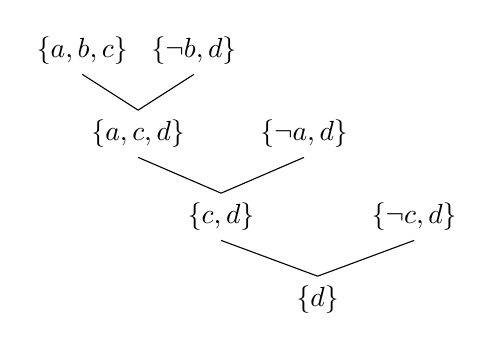
\begin{tikzpicture}[grow'=up]				
				\Tree [.${\{d\}}$ [.${\{c,d \}}$ [.${\{a,c,d\}}$ ${\{a,b,c\}}$ ${\{ \neg b,d\}}$ ]
                           [.${\{ \neg a, d\}}$ ] ]
                           [ .${\{ \neg c, d\}}$  ] ]
       \end{tikzpicture}
	   \caption{A resolution proof for Example \ref{exp:resproof1}.}
	   \label{fig:proof1}
       \end{figure}
\end{examp}

\begin{defi}\label{def:resrefutation}
  A \textbf{resolution refutation} of a clause-set $F$ is a resolution proof deriving $\bot$ from $F$ \cite{h5}. 
\end{defi}
  
Remarks:
\begin{enumerate}
      \item Typically we identify $R$ with $T$, while suppressing $C$.
	  \item Resolution is sound but is incomplete in the sense that it is not guaranteed to derive every clause that is implied by the given $F \in \Cls$. 
	  However, resolution is refutation complete on $\Cls$, i.e., it is guaranteed to derive the empty clause if the given $F$ is unsatisfiable. 
	  This result is the basis for using resolution as a complete algorithm for testing satisfiability: we keep applying resolution until either 
	  the empty clause is derived (unsatisfiable $F$) or until no more applications of resolution are possible (satisfiable $F$) \cite{h6}.
	  \item The number of resolution trees for $F \vdash \bot$ is infinite since we can use any node many times.
	  \item An other definition for \emph{prime implicate} of $F \in \Cls$ is a clause $C$ such that a resolution tree 
	  $T$ with $T: F \vdash C$ exists, but no $T'$ exists for some $C' \subset C$ with $T': F \vdash C'$ \cite{h11}.

\end{enumerate}

 \begin{examp}\label{exp:res1}
      A resolution tree for $F = \{\{a,b\},\{\neg a,b\},\{a, \neg b\},\{\neg a, \neg b\}\}$ is as Fig \ref{fig:resol1}. Since the empty clause 
	  is driven, it is called resolution refutation.
	   \begin{figure}
	   \centering  
       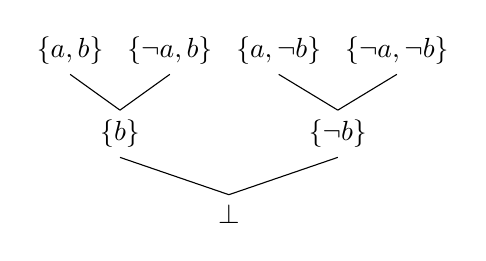
\begin{tikzpicture}[grow'=up]
       \Tree [.$\bot$  [.${\{b\}}$ ${\{a,b\}}$ ${\{\neg a,b\}}$ ]
                           [.${\{ \neg b\}}$ ${\{a, \neg b\}}$ ${\{\neg a, \neg b\}}$ ] ]
       \end{tikzpicture}
	   \caption{A resolution tree for Example \ref{exp:res1}.}
	   \label{fig:resol1}
       \end{figure}
\end{examp}

\begin{examp}\label{exp:res2}
      A resolution tree for $F = \{\{a\},\{\neg a,b\},\{\neg a, \neg b\}\}$ is as Fig \ref{fig:resol2}. Since the empty clause 
	  is driven, it is called resolution refutation.
	  \begin{figure}[h]
       \centering
       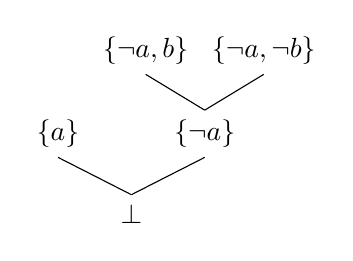
\begin{tikzpicture}[grow'=up]
       \Tree [.$\bot$  [.${\{a\}}$  ]
                           [.${\{ \neg a\}}$ ${\{\neg a, b\}}$ ${\{\neg a, \neg b\}}$ ] ]

       \end{tikzpicture}
	   \caption{A resolution tree for Example \ref{exp:res2}.}
	   \label{fig:resol2}
       \end{figure}
\end{examp}
 
\begin{examp}\label{exp:res3}
      A resolution tree for $F = \{\{\neg a, \neg b\},\{\neg a,b,\neg c, \neg d\},\{a, \neg d\},\{c, \neg d\}, \{d\}\}$ is as 
	  Fig \ref{fig:resol3}. Since the empty clause is driven, it is called resolution refutation.
	\begin{figure}[h]
    \centering
    \begin{forest}
    for tree={
    grow'=90,
    parent anchor=north,
    child anchor=south,
    math content,
    inner xsep=0pt,
    anchor=west,
    before typesetting nodes={
      if level=0{}{
        if content={}{
          shape=coordinate
        }{
          content/.wrap value={\{#1\}},
        },
      },
    },
    if level=0{
      before drawing tree={x=+.5em},
      for children={
        if n=1{
          calign with current,
          edge path={
            \noexpand\path [draw, \forestoption{edge}] (!u.north west) +(.5em,0) coordinate (a) -- (a |- .child anchor)\forestoption{edge label};
          }
        }{
          edge path={
            \noexpand\path [draw, \forestoption{edge}] (!u.north west) +(.5em,0) -- (.child anchor)\forestoption{edge label};
          }
        },
      }
    }{
      for descendants={
        for parent={
          for children={
            if n=1{
              calign with current,
              edge path={
                \noexpand\path [draw, \forestoption{edge}] (!u.north west) +(1em,0) coordinate (a) -- (a |- .child anchor)\forestoption{edge label};
              }
            }{
              edge path={
                \noexpand\path [draw, \forestoption{edge}] (!u.north west) +(1em,0) -- (.child anchor)\forestoption{edge label};
              }
            },
          }
        }
      }
    },
    if n children=0{tier=terminus}{}
  }
  [\bot, tikz={\draw ([xshift=.5em].north west) -- (q.south);}
    [{\neg a}
      [{\neg a, \neg b}]
      [b
        [{b, \neg c}
          [{b, \neg a, \neg c}, tikz={\draw ([xshift=1em].north west) -- (s.south);}
            [{b, \neg a, \neg c, \neg d}]
          ]
          [a, tier=t, name=q, tikz={\draw ([xshift=1em].north west) -- (s.south);}
            [{a, \neg d}]
          ]
        ]
        [c, tier=t
          [{c, \neg d}]
          [d, name=s]
        ]
      ]
    ]
  ]
  \end{forest}
  \caption{A resolution tree for Example  \ref{exp:res3}.}
  \label{fig:resol3}
  \end{figure}
\end{examp}

\begin{defi}\label{def:regres}
  A resolution tree($(T,C)$ (see Definition \ref{def:resproof}) is \textbf{regular} if along every path from the root to some leaf no resolution variable occurs more than once.
\end{defi}
%--------------------------------------------------------------------------------------------------------------------------------------
\section{Reduction}
\label{sec:Reduction}
\begin{defi}\label{def:red}
   A \textbf{reduction} is a map $r: \Cls \ra \Cls$ such that for all $F, F' \in \Cls$ we have
  \begin{enumerate}
  \item $r(F)$ is satisfiability-equivalent to $F$;
  \item if $\bot \in r(F)$ and for all $C \in F$ there is $C' \in  F'$ with $C' \sse C$, then $\bot \in r(F')$.
  \end{enumerate}
  A reduction $r$ \textbf{discovers} unsatisfiability of $F$ if $\bot \in r(F)$ \cite{h10}.
\end{defi}

\begin{defi}\label{def:implication}
  Consider a reduction $r$. The relation $\bmm{F \models_r C}$ holds for a clause-set $F$ and a clause $C$, and we say \textbf{$C$ is deducible from $F$ via $r$}, if $r$ 
  discovers unsatisfiability of $\vp_C * F$ (that is, $\bot \in r(\vp_C * F)$ for $\vp_C = \pab{x \mapsto 0 : x \in C}$).
\end{defi}
%--------------------------------------------------------------------------------------------------------------------------------------
\section{Generalised unit-clause-propagation}
\label{sec:rkred}

An important special case of resolution is called \textbf{unit resolution (unit propagation)}. Unit resolution is a resolution strategy 
which requires that at least one of the resolved clauses has only one literal. Such clause is call a \textbf{unit clause}. Unit resolution 
is not refutation complete, which means that it may not derive the empty clause from an unsatisfiable CNF formula. Yet one can apply all 
possible unit resolution steps in time linear in the size of given CNF. Because of its efficiency, unit resolution is a key technique 
employed by a number of algorithms \cite{h6}.

The unit resolution technique (or unit propagation) is quite simple: first, we close the CNF under unit resolution and collect all unit 
clauses in the CNF. We then assume that variables are set to satisfy these unit clauses. That is, if the unit clause $\{x\}$ appears 
in the CNF, we set $x$ to true. And if the unit clause $\{\neg x\}$ appears in the CNF, we set $x$ to false. We then simplify the 
CNF given these settings and check for either success (all clauses are subsumed) or failure (the empty clause is derived)\cite{h6}.

\begin{examp}\label{exp:unit1}
      Let $F=\{ \{a\}, \{a, b\}, \{\neg a, c\}, \{\neg c, d\}\}$. By unit propagation (because $F$ contains the unit clause $\{a\}$), 
	  we obtain $\varphi_a * F=\langle a \rightarrow 1 \rangle * F= \{ \{c\}, \{\neg c, d\}\}$. If $\bot \in \varphi_a * F$, then $F$ is 
	  satisfiability-equivalent to $\varphi_a * F$ and we eliminated one variable. Otherwise, we know that all clauses in $\varphi_a * F$ 
	  must have length at least 2. So, in this case $F$ is also satisfiability equivalent to $\varphi_a * F$, and again at least one 
	  variable has been eliminated.
\end{examp}

\begin{defi}\label{def:rk}
  The maps $\bmm{\rk_k}: \Cls \ra \Cls$ for $k \in \NNZ$ are defined as follows (for $F \in \Cls$):
  \begin{eqnarray*}
    \rk_0(F) & := &
    \begin{cases}
      \set{\bot} & \text{if } \bot \in F\\
      F & \text{otherwise}
    \end{cases}\\
    \rk_{k+1}(F) & := &
    \begin{cases}
      \rk_{k+1}(\pao x1 * F) & \text{if } \ex\, x \in \lit(F) : \rk_k(\pao x0 * F) = \set{\bot}\\
      F & \text{otherwise}
    \end{cases}.
  \end{eqnarray*}
\end{defi}
Remarks:
\begin{enumerate}
\item $\rk_1$ is unit-clause propagation, $\rk_2$ is (full) failed literal elimination.
\item In general we can call $\rk_k$ \textbf{$k$-propagation-reduction} or \textbf{generalised unit-clause-propagation of level $k$}.
\end{enumerate}

\begin{examp}\label{exp:rk}
  Computing some $\rk_k(F)$, using literals $x,y,x_1,\dots,x_n$ ($n \in \NNZ$) with distinct underlying variables:
  \begin{enumerate}
  \item $\rk_k(\set{\bot}) = \set{\bot}$ for $k \ge 0$.
  \item $\rk_k(\top) = \top$ for $k \ge 0$.
  \item For $F := \set{\set{x_1},\dots,\set{x_n}}$: $\rk_0(F) = F$, $\rk_k(F) = \top$ for $k \ge 1$.
  \item For $F' := F \cup \set{\set{x,y}}$: $\rk_0(F') = F'$, $\rk_k(F') = \set{\set{x,y}}$ for $k \ge 1$ (note that $\set{\set{x,y}}$ has no forced assignments).
  \item For $F := \set{\set{x,y},\set{x,\ol{y}}}$: $\rk_k(F) = F$ for $k \le 1$, $\rk_k(F) = \top$ for $k \ge 2$.
  \item For $F := \set{\set{x,y},\set{x,\ol{y}}, \set{\ol{x},y},\set{\ol{x},\ol{y}}}$: $\rk_k(F) = F$ for $k \le 1$, $\rk_k(F) = \set{\bot}$ for $k \ge 2$.
  \end{enumerate}
\end{examp}

%--------------------------------------------------------------------------------------------------------------------------------------
\section{Horton-Strahler number}
\label{sec:hs}
\begin{defi}\label{def:hdtree}
  Consider a resolution tree $T$ (recall Definition \ref{def:resproof}). The \textbf{Horton-Strahler} number $\bmm{\hts(T)} \in \NNZ$ 
  is defined as $\hts(T) := 0$, if $T$ is trivial (consists only of one node), while otherwise we have two subtrees $T_1, T_2$, and 
  we set $\hts(T) := \max(\hts(T_1),\hts(T_2))$ if $\hts(T_1) \not= \hts(T_2)$, while in case of $\hts(T_1) = \hts(T_2)$ we set $\hts(T) := \max(\hts(T_1),\hts(T_2)) + 1$.
\end{defi}

\begin{examp}\label{exp:hortonstrahler}
  Fig \ref{fig:hst} showes some examples of trees with their Horton-Strahler numbers. We denote by $T_1$ and $T_2$ in each example the left and right sub-trees of the root.
 \begin{figure}[h] 
  \begin{center}
  %\centring
    \begin{tabular}{|>{\centering\arraybackslash}m{10em}|>{\centering\arraybackslash}m{3em}|>{\centering\arraybackslash}m{7em}|}
      \hline
      \textbf{Tree $T$} & \bmm{\hts(T)} & \textbf{Explanation} \\\hline\hline
      $\displaystyle
      \xygraph{
        []{\cdot} ( )
      }$ & 0 & trivial tree \\ \hline
      $\displaystyle
      \xygraph{
        !{0;/r3ex/:}
        []{\cdot} (
          - [dl]{\cdot} (),
          - [dr]{\cdot} ()     )
      }$ & 1 & $\hts(T_1) = 0$, $\hts(T_2) = 0$. \\ \hline
      $\xygraph{
        !{0;/r3ex/:}
        []{\cdot} (
        - [dl]{\cdot} (),
        - [dr]{\cdot} (
          -[dl]{\cdot} (),
          -[dr]{\cdot} ()   )    )
      }$ & 1 & $\hts(T_1) = 0$, $\hts(T_2) = 1$.  \\ \hline
      $\xygraph{
        !{0;/r3ex/:}
        []{\cdot} (
          - [dl]{\cdot} (),
          - [dr]{\cdot} (
            -[dl]{\cdot} (),
            - [dr]{\cdot} (
              -[dl]{\cdot} (),
              -[dr]{\cdot} ()      )    )    )
      }$ & 1 & $\hts(T_1) = 0$, $\hts(T_2) = 1$.  \\ \hline
      $\xygraph{
        !{0;/r3ex/:}
        []{\cdot} (
        - [dll]{\cdot} (
          -[dl]{\cdot} (),
          -[dr]{\cdot} ()     ),
        - [drr]{\cdot} (
          -[dl]{\cdot} (),
          -[dr]{\cdot} ()    )    )
      }$ & 2 & $\hts(T_1) = 1$, $\hts(T_2) = 1$.  \\ \hline
      $\xygraph{
        !{0;/r3ex/:}
        []{\cdot} (
        - [dll]{\cdot} (
          -[dl]{\cdot} (),
          -[dr]{\cdot} ()     ),
        - [drr]{\cdot} (
          -[dll]{\cdot} (
            -[dl]{\cdot} (),
            -[dr]{\cdot} ()   ),
          -[dr]{\cdot} (
            -[dl]{\cdot} (),
            -[dr]{\cdot} ()   )   )    )
      }$ & 2 & $\hts(T_1) = 1$, $\hts(T_2) = 2$.  \\ \hline
    \end{tabular}
  \end{center}
  \caption{Horton-Strahler numbers of some trees.}
  \label{fig:hst}
  \end{figure}
\end{examp}
%--------------------------------------------------------------------------------------------------------------------------------------
\section{Hypergraph}
\label{sec:hpg}

\begin{defi}\label{def:hypergraphs}
  A \textbf{hypergraph} is a pair $G=(V,E)$, where $V$ is a set (the set of ``vertices''), while $E \sse \pote(V)$ is a set of finite subsets of $V$ (the ``hyperedges''). 
  We use for a hypergraph $G = (V,E)$ the notations $\bmm{V(G)} := V$ and $\bmm{E(G)} := E$. A general hypergraph is a triple $(V,E,e)$ where $V, E$ are sets and $e:E \rightarrow \pot_f(V)$ 
  where $\pot_f(V)$ for a set $X$ is the set of finite subsets of $X$: one writes $e(G)=e$ \cite{h5}. 
\end{defi}

\begin{examp}\label{exp:hypergraph1}
      Fig \ref{fig:hypergraph1} showes an example of hypergraph with $V=\{ v_1, v_2, v_3, v_4, v_5, v_6, v_7 \}$ and $E=\{ e_1, e_2, e_3, e_4\} = \{ \{ v_1, v_2, v_3\}, \{v_2, v_3\}, \{ v_3, v_5, v_6\}, \{ v_4 \}\}$.
	   
	\begin{figure}[h]
    \centering  
	\begin{tikzpicture}
    \node (v1) at (0,2) {};
    \node (v2) at (1.5,3) {};
    \node (v3) at (4,2.5) {};
    \node (v4) at (0,0) {};
    \node (v5) at (2,0.5) {};
    \node (v6) at (3.5,0) {};
    \node (v7) at (2.5,-1) {};
    \begin{scope}[fill opacity=0.8]
    \filldraw[fill=yellow!70] ($(v1)+(-0.5,0)$) 
        to[out=90,in=180] ($(v2) + (0,0.5)$) 
        to[out=0,in=90] ($(v3) + (1,0)$)
        to[out=270,in=0] ($(v2) + (1,-0.8)$)
        to[out=180,in=270] ($(v1)+(-0.5,0)$);
    \filldraw[fill=blue!70] ($(v4)+(-0.5,0.2)$)
        to[out=90,in=180] ($(v4)+(0,1)$)
        to[out=0,in=90] ($(v4)+(0.6,0.3)$)
        to[out=270,in=0] ($(v4)+(0,-0.6)$)
        to[out=180,in=270] ($(v4)+(-0.5,0.2)$);
    \filldraw[fill=green!80] ($(v5)+(-0.5,0)$)
        to[out=90,in=225] ($(v3)+(-0.5,-1)$)
        to[out=45,in=270] ($(v3)+(-0.7,0)$)
        to[out=90,in=180] ($(v3)+(0,0.5)$)
        to[out=0,in=90] ($(v3)+(0.7,0)$)
        to[out=270,in=90] ($(v3)+(-0.3,-1.8)$)
        to[out=270,in=90] ($(v6)+(0.5,-0.3)$)
        to[out=270,in=270] ($(v5)+(-0.5,0)$);
    \filldraw[fill=red!70] ($(v2)+(-0.5,-0.2)$) 
        to[out=90,in=180] ($(v2) + (0.2,0.4)$) 
        to[out=0,in=180] ($(v3) + (0,0.3)$)
        to[out=0,in=90] ($(v3) + (0.3,-0.1)$)
        to[out=270,in=0] ($(v3) + (0,-0.3)$)
        to[out=180,in=0] ($(v3) + (-1.3,0)$)
        to[out=180,in=270] ($(v2)+(-0.5,-0.2)$);
    \end{scope}
    \foreach \v in {1,2,...,7} {
    \fill (v\v) circle (0.1);    }
    \fill (v1) circle (0.1) node [right] {$v_1$};
    \fill (v2) circle (0.1) node [below left] {$v_2$};
    \fill (v3) circle (0.1) node [left] {$v_3$};
    \fill (v4) circle (0.1) node [below] {$v_4$};
    \fill (v5) circle (0.1) node [below right] {$v_5$};
    \fill (v6) circle (0.1) node [below left] {$v_6$};
    \fill (v7) circle (0.1) node [below right] {$v_7$};
    \node at (0.2,2.8) {$e_1$};
    \node at (2.3,3) {$e_2$};
    \node at (3,0.8) {$e_3$};
    \node at (0.1,0.7) {$e_4$};
    \end{tikzpicture}
    \caption{An example of hypergraph.}
    \label{fig:hypergraph1}
    \end{figure}
\end{examp}
%***************************************************************************************************************************************************************
%***************************************************************************************************************************************************************
\chapter{Hardness measures}
\label{cha:Hardness Measures}

Hardness $h :\Cls \rightarrow \NNZ$ is a measure for SAT representation "complexity". In this chapter, first two hardness 
measures for ustatisfiable clause-sets are defined as $ h_0 : \Usat \rightarrow \NNZ$ for unsatisfiable $F$.
Then, in section \ref{sec:extension_Hardness} and \ref{sec:extensionWidth-hardness} these measures are extended to arbitrary 
cluase-set $F \in \Cls$. The basic idea according to \cite{h20} is to consider the hardness 
of unsatisfiable sub-instances, obtained by partial instantiations. Then, the worst-case situation is considered which yields 
precise measurements. However, there are various equivalent descriptions for hardness in the literature. 

%--------------------------------------------------------------------------------------------------------------------------------------
\section{Tree-hardness of unsatisfiable clause-sets}
\label{sec:Hardnessunsat}

The tree-hardness (or just hardness) measures the height of the biggest full binary tree which can be embedded into each tree-like resolution 
refutation of the formula. This is also known as the Horton-Strahler number of a tree. There is another equivalent description, 
which uses generalised unit-clause propagation $r_k$ to measure hardness. Following, the definition based on Horton-Strahler number is presented.

\begin{defi}\label{def:hardness1}
      \cite{h5} For $F \in \Usat$ let \textbf{hardness} $\bmm{\hardness(F)} \in \NNZ$ be the minimal $k \in \NNZ$ such that a resolution tree $T : F \vdash \bot$ 
	  exists, where the Horton-Strahler number of $T$ is at most $k$. For $k \in \NNZ$ let $\Urefc_k  := \{F \in \Cls : \hardness(F) \le k\}$ .
\end{defi}
And another description which uses generalised unit-clause propagation $r_k$ to measure hardness is:
\begin{defi}\label{def:hardness2}
  \cite{h13} The \textbf{hardness} $\hardness(F)$ of an unsatisfiable $F \in \Cls$ is the minimal $k \in \NNZ$ such that $\rk_k(F) = \set{\bot}$.
\end{defi}

\begin{examp}\label{exp:hardness1}
      For $\set{\set{x,y},\set{x,\ol{y}},\set{\ol{x},y},\set{\ol{x},\ol{y}}}$ we have $r_1(F)=F, r_2(F)=r_2( \langle a \rightarrow 1 \rangle * F) = \{ \bot \}$
	  (since $r_1( \langle a \rightarrow 0 \rangle * F)=r_1 (\{\{ b \}, \{ \neg b \}\}) = \{ \bot \}$). Thus, $\hardness(F) = 2$.
\end{examp}

\begin{examp}\label{exp:harducls}
  Here are some basic determinations of $\hardness(F)$ for unsatisfiable clause-sets $F$, using literals $x,y,z$ with distinct underlying variables:
  \begin{enumerate}
  \item $\hardness(F) = 0$ iff $\bot \in F$.
  \item $\hardness(\set{\set{x},\set{\ol{x}}}) = 1$.
  \item $\hardness(\set{\set{x},\set{\ol{x},y}, \set{\ol{y},z}, \set{\ol{z}}}) = 1$.
  \item $\hardness(\set{\set{x,\ol{y}},\set{\ol{x},y},\set{y,\ol{z}},\set{\ol{y},z},\set{x,y,z},\set{\ol{x},\ol{y},\ol{z}}}) = 2$.
  \end{enumerate}
\end{examp}
There is also a simple measure for hardness called depth.
\begin{defi}\label{def:hardness2}
      \cite{h5} For $F \in \Usat$ let $\textbf{dep(F)} \in \NN_0$ be the minimal height of a resolution tree $T : F \vdash \bot$.
\end{defi}

Remarks:
\begin{enumerate}
  \item Since the Horton-Strahler number of a tree is at most the height, we get $\hardness(F) \le dep(F)$ for all $F \in \Cls$.
\end{enumerate}
%--------------------------------------------------------------------------------------------------------------------------------------
\section{Extension of tree-hardness to satisfiable clause-sets}
\label{sec:extension_Hardness}

As it is mentioned before, in this section the hardness measure is extended to arbitrary clause-set (both satisfiable and unsatisfiable). 

\begin{defi}\label{def:ex-hardness}
\cite{h11} The hardness $\hardness : \Cls \rightarrow \NNZ$ is defined for $F \in \Cls$ as follows:
\begin{enumerate}
  \item If $F \in \Usat$ , then $\hardness(F)$ is the minimum hs(T) for $T : F \vdash \bot$.
  \item If $F = \top$, then $\hardness(F) := 0$.
  \item If $F \in \Sat \ \{ \top \}$, then $\hardness(F) := \max \{ \hardness(\varphi * F) : \varphi * F \in \Usat \}$.
  \end{enumerate}
\end{defi}
\begin{quest}\label{que:hardness_measures}
      Is there any relation among various hardness measures?
\end{quest}
%--------------------------------------------------------------------------------------------------------------------------------------
\section{Width-hardness of unsatisfiable clause-sets}
\label{sec:whdd}

Another measure for SAT representation complexity is called width-hardness or resolution-width. The standard resolution-width of an 
unsatisfiable clause-set $F$ is the minimal $k$ such that a resolution refutation of $F$ using only clauses of length at most $k$ exists \cite{h20}.

\begin{defi}\label{def:whd1}
     \cite{h5} For  $F \in \Usat$ the \textbf{symmetric width} $\bmm{\wid(F)} $\in \NNZ$ is the smallest $k \in \NNZ$ such that there is
	 $T : F \vdash \bot$ with $\widehat{F}(T) \in k-\Cls$.
\end{defi}
\begin{defi}\label{def:whd2}
  \cite{h5} For a resolution tree $T$ its \textbf{(asymmetric) width} $\bmm{\whardness(T)} \in \NNZ$ is defined as $0$ if $T$ is trivial 
  (i.e., $\abs{\nds(T)} = 1$), while otherwise for left and right children $w_1, w_2$ with subtrees $T_1, T_2$ we define
  \begin{displaymath}
    \whardness(T) := \max \big (\whardness(T_1), \whardness(T_2), \, \min(\abs{C(w_1)}, \abs{C(w_2)}) \big )
  \end{displaymath}
  (note that the corresponding definition of $\wid(T)$ just has the $\min$ replaced by a (second) $\max$). We write \bmm{R : F \vdash^k C} if $R : F \vdash C$ and $\whardness(R) \le k$. 
  Now for $F \in \Usat$ we define $\bmm{\whardness(F)} := \min \set{\whardness(T) \mb T : F \vdash \bot}\in \NNZ$. For $k \in \NNZ$ let $\bmm{\Wrefc_k} := \set{F \in \Cls : \whardness(F) \le k}$.
\end{defi}
Remarks:
	    \begin{enumerate}
              \item For all $F \in \Cls $ holds $\whardness(F)$ \le \hardness(F)$.
		\end{enumerate}
\begin{examp}\label{exp:whd1}
      \cite{h5} Some examples for $\wid(F)$ and $\whardness(F)$ are as below:
	    \begin{enumerate}
              \item $\wid(\set{\bot}) = \whardness(\set{\bot}) = 0$.
			  \item More generally for $C \in \Cl$ holds $wid(\{C\}) = \whardness(\{C\}) = 0$.
			  \item In general we have $\wid(F) = 0 \Leftrightarrow \whardness(F) = 0$ for all $F \in \Cls$.
			  \item For a Horn clause-set $F$ holds $\whardness(F) \le 1$ (since unit-clause propagation is sufficient to derive unsatisfiability), 
			  while $\wid(F)$ is unbounded (if $F$ is minimally unsatisfiable, then $\wid(F)$ equals the maximal clause-length of $F$).
			  \item For general minimally unsatisfiable $F$, the maximal clause-length is a lower bound for $\wid(F)$, but is unrelated to 
			  $\whardness(F)$.
      	\end{enumerate}		  
\end{examp}

\begin{examp}\label{exp:whd2}
      For $F := \{\{a\}, \{a, b\}, \{a, b\}\}$ there are two possible trees as $T_1$ in Fig \ref{fig:whd2} and $T_2$ in Fig \ref{fig:resol2}.   
	  Using Definition \ref{def:whd2}, we have $\whardness(T_1) = 1$ and $\whardness(T_2) = 2$ and finally $\whardness(F) = 1$. $\wid(F) = 2$ is also 
	  obtained by Definition \ref{def:whd1}.
	  \begin{figure}
      \begin{center}
	  %\centering
      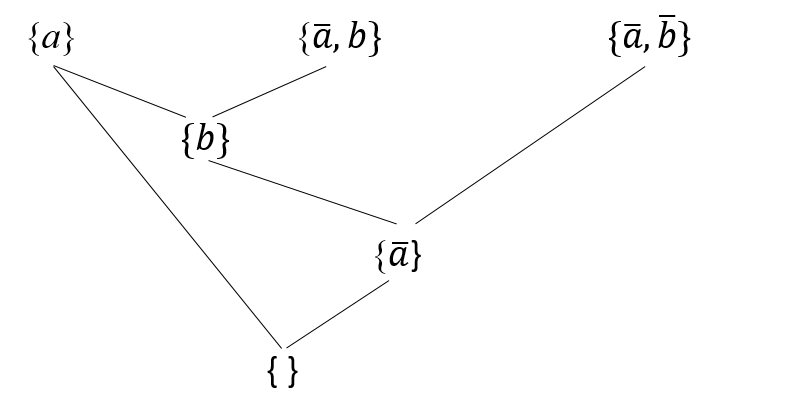
\includegraphics[scale =0.6]{whd1.png}
      \caption{The esolution tree $T_1$ in \ref{exp:whd2}.}
	  \label{fig:whd2}
      \end{center}
      \end{figure}
\end{examp}
%--------------------------------------------------------------------------------------------------------------------------------------
\section{Extension of width-hardness to satisfiable clause-sets}
\label{sec:extensionWidth-hardness}
Here, the width-hardness measure is extended to arbitrary clause-set (both satisfiable and unsatisfiable). 

\begin{defi}\label{def:ex-whd}  
      \cite{h11} The \textbf{width-hardness} $\whardness : \Cls \rightarrow \NNZ$  is defined for $F \in \Cls$ as follows:
	  \begin{enumerate}
              \item If $F \in \Usat$ , then $\whardness(F)$ is the minimum $k \in \NNZ$ such that k-resolution refutes $F$, that is, such that
			  $T : F \vdash \bot$ exists where for each resolution step $R = C  \diamond D$ in $T$ we have $ \abs{C } \le k$ or $\abs{D } \le k$.
			  \item If $F = \top$, then $\whardness(F) := 0$.
			  \item If $F \in \Sat \ \{ \top \}$, then $\whardness(F) := \max \{\whardness(\varphi * F) : \varphi * F \in \Usat\}$.
      \end{enumerate}
\end{defi}

%***************************************************************************************************************************************
%***************************************************************************************************************************************************************
\chapter{XOR representation}
\label{cha:XOR-representation}

\section{XOR-clause-sets}
\label{sec:xor-cls}

\begin{defi}\label{def:xor-const} 
      \cite{h8} An \textbf{XOR-constraint} (also known as ``parity constraint'') is a (boolean) constraint of the form $x_1 \oplus \dots \oplus x_n = \ve$ 
	  for literals $x_1, \dots, x_n$ and $\ve \in \set{0,1}$, where $\oplus$ is the addition in the 2-element field $\ZZ_2 = \set{0,1}$. 
\end{defi}
Remarks:
\begin{enumerate}
      \item $x_1 \oplus \dots \oplus x_n = y$ is equivalent to $x_1 \oplus \dots \oplus x_n \oplus y = 0$
	  \item $x \oplus x = 0$, $x \oplus \ol{x} = 1$, $0 \oplus x = x$, $1 \oplus x = \ol{x}$.
	  \item Two XOR-constraints are \emph{equivalent}, if they have exactly the same set of solutions.
\end{enumerate}
Now, a representation that uses  this XOR-constraints is presented.	In this representation, ordinary clauses $C \in \Cl$ are 
implicitly interpreting as the XOR-constraints $\oplus_{x \in C} = 0$.  

\begin{defi}\label{def:xor-cls}
      \textbf{XOR-clause-sets} $F$ are sets of XOR-clauses, that is, ordinary clause-sets $F \in \Cls$ with a different interpretation. 
	  So two XOR-clauses $C, D$ are equivalent iff $\var(C) = \var(D)$ and the number of complements in $C$ has the same parity as the 
	  number of complements in $D$.
\end{defi}
Remarks:
\begin{enumerate}
      \item Clashing literal pairs can be removed by $x \oplus \ol{x} = 1$ and $1 \oplus y = \ol{y}$.
	  \item Every XOR-constraint can be represented by an XOR-clause except of inconsistent XOR-constraints, 
	  where the simplest form is $0=1$; we can represent this by \emph{two} XOR-clauses $\set{v}, \set{\ol{v}}$ \cite{h8}.
	  \item A partial assignment $\vp \in \Pass$ satisfies an XOR-clause-set $F$ iff $\var(\vp) \supseteq \var(F)$ and for 
	  every $C \in F$ the number of $x \in C$ with $\vp(x) = 1$ is even \cite{h8}. 
	  \item An XOR-clause-set $F$ implies an XOR-clause $C$ if every satisfying partial assignment $\vp$ for $F$ is also a 
	  satisfying assignment for $\set{C}$ \cite{h8}.  
\end{enumerate}

\begin{defi}\label{def:cnfrepxor} 
  \cite{h8} A \textbf{CNF-representation} of an XOR-clause-set $F \in \Cls$ is a clause-set $F' \in \Cls$ with $\var(F) \sse \var(F')$, 
  such that the projections of the satisfying total assignments for $F'$ (as CNF-clause-set) to $\var(F)$ are precisely the satisfying 
  (total) assignments for $F$ (as XOR-clause-set).
\end{defi}
According to literature, it is costly to obtain the CNF-representation of an XOR-clause-set. So, it is not the case in this report. 
Now, there are two questions. The first question is how to determine whether an XOR-clause-set is satisfiable or not and the
second one is how to abtain a CNF-representation of an XOR-clause-set. The first question is answered as follows and the second 
one in investigated in Section \ref{sec:x0}.
At first, we need to define the operation of XOR-sum over XOR-clauses which operates as the resolution operation for CNF-clauses.
Then, we define the satisfiability using this operation.

\begin{defi}\label{def:xorsum}
  \cite{h8} Consider an XOR-clause-set $F \in \Cls$. We define the partial operation \textbf{XOR-sum over clauses of $F$}, written 
  as $\bmm{\oplus F} \in \Cl$, as the reduction of $\symdif_{C \in F} C$ via the basic XOR-rules to some clause $\oplus F := E \in \Cl$, 
  assuming that the reduction does not end up in the situation $E = \set{v,\ol{v}}$ for some variable $v$ --- in this case we say that 
  $\oplus F$ is inconsistent (which is only possible for $c(F) \ge 2$).

  The reduction, starting with the XOR-pseudo-clause $\symdif_{C \in F} C$, and either producing $\oplus F \in \Cl$ or resulting in 
  ``inconsistent'', proceeds as follows:
  \begin{enumerate}
  \item First all quadruples $v,\ol{v},w,\ol{w}$ for variables $v \ne w$ are removed (due to $x \oplus \ol{x} = 1$ and $1 \oplus 1 = 0$).
  \item If no clash remains, then we obtained the result $E \in \Cl$.
  \item If a single pair $v, \ol{v}$ remains, and there is at least one other literal $x$ left, then $v, \ol{v}$ is removed, and 
  according to some choice-rule one such remaining literal $x$ is chosen and replaced by $\ol{x}$ (due to $1 \oplus x = \ol{x}$), 
  obtaining the result $E \in \Cl$.
  \item But if only a pair $v, \ol{v}$ remains (no other literal), then we have the situation that $\oplus F$ is inconsistent.
  \end{enumerate}
\end{defi}

\begin{examp}\label{exp:xorcls2}
  \cite{h8} For the following computation we consider only variables from $\NN$, and assume that the chosen literal $x$ is the 
  one with minimal $\var(x)$:
  \begin{enumerate}
  \item $\oplus \top = \oplus(\set{\bot}) = \bot$ (note that as an XOR-clause, $\bot$ is a tautology).
  \item $\oplus \set{\set{1,2},\set{2,3}} = \set{1,3}$.
  \item $\oplus \set{\set{1,2,-3},\set{-1,2,3}} = \bot$.
  \item $\oplus \set{\set{1,2},\set{-1,2}}$ is inconsistent.
  \item $\oplus \set{\set{1,2,-3,4},\set{-1,2,3,-4,5,6}} = \set{-5,6}$.
  \end{enumerate}
\end{examp}

\begin{lem}\label{lem:characimplxor}
  \cite{h8} Consider an XOR-clause-set $F \in \Cls$. $F$ is unsatisfiable if and only if there is $F' \sse F$ such that $\oplus F'$ is inconsistent.

\end{lem}
%--------------------------------------------------------------------------------------------------------------------------------------
\section{$\bmm{X_0}$ translation}
\label{sec:x0}

In this section, a method to obtain the CNF-representation of an XOR-clause-set is presented. The translation $X_0(F)$ 
translates an XOR-clause-set by the unique equivalent CNF-clause-set. Here, the question is that whether this equivalent clause-set 
is unique or not. The answer is that there is precisely one CNF-clause-set equivalent to the XOR-clause-set $\set{C}$ according 
to its definition.

\begin{defi}\label{def:x0def} 
The \textbf{translation} $\bmm{X_0(F)}$ is the set of prime implicates of the underlying boolean function i.e., 
\begin{displaymath}
  \bmm{X_0(C)} := \primec_0(x_1 \oplus \dots \oplus x_n = 0) \in \Urefc_0.
\end{displaymath}
and is unique since the prime implicates are not resolvable (and are full, 
so that not even subsumptions are possible).

$X_0(C)$ has $2^{n-1}$ clauses for $n \ge 1$ (while for $n=0$ we have $X_0(C) = \top$), namely the full clauses (containing all variables) 
over $\set{\var(x_1),\dots,\var(x_n)}$, where the parity of the number of complementations is different from the parity of the number of 
complementations in $C$ \cite{h8}.
\end{defi}

\begin{examp}\label{exp:X0}
  \cite{h8} $X_0(\set{1,2}) = \set{\set{-1,2},\set{1,-2}}$, $X_0(\set{1,-2}) = \set{\set{1,2},\set{-1,-2}}$.
\end{examp}

Remarks:
\begin{enumerate}
  \item For two XOR-clauses $C, D$ we have $X_0(C) = X_0(D)$ iff $C, D$ are equivalent.
  \item More generally, we define $X_0: \Cls \ra \Cls$, where the input is an XOR-clause-set and the output is a CNF-clause-set, 
  by $\bmm{X_0(F)} := \bc_{C \in F} X_0(C)$.
  
\end{enumerate}  

\begin{examp}\label{exp:2xor0}
  \cite{h8} For $n \in \NN$ and (different) variables $v_1,\dots,v_n$ consider the system
  \begin{eqnarray*}
    v_1 \oplus v_2 \oplus \dots \oplus v_n &=& 0 \\
    v_1 \oplus v_2 \oplus \dots \oplus \ol{v_n} &=& 0,
  \end{eqnarray*}
  that is, consider the XOR-clauses $C_1 := \set{v_1,\dots,v_n}$ and $C_2 := \set{v_1,\dots,v_{n-1},\ol{v_n}}$. Then $X_0(\set{C_1,C_2})$ 
  is the clause-set with all $2^n$ full clauses over $\set{v_1,\dots,v_n}$. It follows $\hardness(X_0(\set{C_1,C_2})) = \whardness(X_0(\set{C_1,C_2})) = n$ (due to the minimal 
  clause-length $n$ we have $n \le \whardness(X_0(\set{C_1,C_2}))$, while due to the variable-number $n$ we have $\hardness(X_0(\set{C_1,C_2})) \le n$).
\end{examp}


%--------------------------------------------------------------------------------------------------------------------------------------
\section{The Tseitin clause-sets}
\label{sec:Tseitin cls}

Consider a general graph $G = (V,E,\eta)$, that is, $V$ is the set of vertices, $E$ is the set of edge-labels, while 
$\eta: E \ra \set{e \sse V : 1 \le \abs{e} \le 2}$ maps every edge-label $x$ to some edge $\eta(x)$ (so parallel edges and loops are allowed). 
Additionally we demand:
\begin{itemize}
\item $E$ is a clause; thus edge-labels are also literals, and we may speak of ``literal-edges''.
\item There is a ``charge'' $\rho: V \ra \set{0,1}$.
\end{itemize}
We want only to deal with XOR-clauses, and so we forbid the case that an isolated vertex can have charge $1$ (that would lead to ``$0 = 1$''; 
otherwise $\rho$ is arbitrary). For every vertex $w \in V(G)$ the XOR-clause $C_w \in \Cl$ is defined via the equation
\begin{displaymath}
  \oplus_{x \in E(G), w \in \eta(x)} \; x = \rho(w),
\end{displaymath}
that is, the XOR over all literal-edges incident with $w$ is $\rho(w)$. Let
\begin{displaymath}
  T_0(G,\rho) := \set{C_w : w \in V(G)} \in \Cls
\end{displaymath}
be the XOR-clause-set derived from $G$. Then $T_0(G,\rho)$ is unsatisfiable if $G$ has no loops and  $\oplus_{w \in V(G)} \rho(w) = 1$, since 
$\oplus_{w \in V(G)} \oplus_{x \in E(G), w \in \eta(x)} x = 0$, due to every edge occurring precisely twice in the sum. Finally the 
\textbf{Tseitin clause-set} is $T(G,\rho) := X_0(T_0(G,\rho))$; typically we just use ``$T(G)$'' \cite{h8}.

\begin{examp}\label{exp:2xor0T}
  \cite{h8} For an XOR-clause $C$ we have $X_0(C) = T(B_C)$, where $B_C$ is the ``bouquet'' (a general graph with one vertex) with the (single) vertex 
  $C$, which has charge $0$, and the literals of $C$ as edges (loops).

  To obtain the translation of the two XOR-clauses $C_1, C_2$ from Example \ref{exp:2xor0}, we consider the dipole $D_n$, which is the general 
  graph with two vertices and the variables $v_1,\dots,v_n$ as edges connecting these two vertices, where the first vertex gets charge $0$ and 
  the second gets charge $1$. We have $X_0(\set{C_1,C_2}) = T(D_n)$.
\end{examp}
%-----------------------------------------------------------------------------------------
Another way to obtain Tseitin graph is using the Definition \ref{def:hypergraphs} for hypergraph according to \cite{h5}. 
In this case, we conside a system of XOR-constraints/linear equations which is a pair $(G,\rho)$, where $G$ is a finite hypergraph with 
$V(G) \sse \Va$, and $\rho: E(G) \ra \set{0,1}$ assigns to each hyperedge (an equation) the prescribed sum. The basic associated 
clause-set is $\bmm{X_0(G,\rho)} \in \Cls$ defined as
\begin{displaymath}
  X_0(G,\rho) := X_0(\set{\oplus_{v \in H} = \rho(H)}_{H \in E(G)}).
\end{displaymath}

The \textbf{dual} of $(G,\rho)$, written $\trans{(G,\rho)}$, is the pair $(\trans{G}, \rho)$, where
\begin{itemize}
\item $\trans{G}$ is the dual of $G$ as general hypergraph, that is:
  \begin{itemize}
  \item $V(\trans{G}) = E(G)$
  \item $E(\trans{G}) = V(G)$
  \item the hyperedge-function $e: E(\trans{G}) \ra \pote(V(\trans{G}))$ assigns to every $v \in V(G)$ the set of $H \in E(G)$ with $v \in H$;
  \end{itemize}
\item so now $\rho: V(\trans{G}) \ra \set{0,1}$.
\end{itemize}
In general, a \emph{dual system of XOR-constraints/linear equations over $\ZZ_2$} is a pair $(G,\rho)$, where $G$ is a finite general hypergraph 
with $E(G) \sse \Va$ and $\rho: V(G) \ra \set{0,1}$. So the associated system of XOR-constraints is obtained again by dualisation, written again 
$\trans{(G,\rho)} := (\trans{G},\rho)$, where $\trans{G}$ is the dual of $G$ as (ordinary) hypergraph, that is, $V(\trans{G}) = E(G)$ and $E(\trans{G}) = \set{v \in E(G) : w \in e(G)(v)}_{w \in V(G)}$. 
The associated clause-set $\bmm{X_0(G,\rho)} \in \Cls$ is $X_0(G,\rho) := X_0(\trans{(G,\rho)})$.

Obviously dualisation in both directions yields inverse bijections between the set of systems of XOR-constraints and the set of dual systems of XOR-constraints \cite{h5}.

\begin{defi}\label{def:tgraph}
\cite{h5} A \textbf{full Tseitin graph} is a dual system of XOR-constraints $(G,\rho)$, where $G$ is a connected irreflexive general graph with 
$\oplus_{w \in V(G)} \rho(w) = 1$, where irreflexive general graphs says $\fa\, v \in E(G) : \abs{e(G)(v)} = 2$. Note that additionally to ordinary (
full) Tseitin graphs we allow parallel edges, but still loops are disallowed (a loop at a vertex in effect deactivates the corresponding equation). 
Now $X_0(G,\rho) \in \Usat$ .
\end{defi}

An important abstraction is obtained by the insight, that $X_0(G,\rho)$ and $X_0(G,\rho')$ are flipping-isomorphic, that is, by flipping literals we 
can obtain the former from the latter. So we consider plain connected irreflexive general graph with at least one vertex as \textbf{Tseitin graphs}, 
considering implicitly the set of all possible vertex-labellings (with elements from $\set{0,1}$, so that the (XOR-)sum is $1$).

To understand $\hardness(X_0(G))$ and $\whardness(X_0(G))$, we need to understand what splitting does with $G$. 
The variables $v \in \var(F)$ of $F := X_0(G)$ are the edges of $G$:
\begin{itemize}
\item If $G' := G - v$ is still connected, then $\pao v0 * F$ and $\pao v1 * F$ are both isomorphic to $X_0(G')$. Note that $G'$ is still a Tseitin graph.
\item Otherwise let $G', G''$ be the connected components of $G$ (both again Tseitin graphs). Now $\pao v0 * F$ and $\pao v1 * F$ are isomorphic, in some 
order, to $X_0(G'), X_0(G'')$.
\end{itemize}
The endpoint of splitting is reached when $G$ is the one-point graph (which can not have edges, since loops are not allowed) \cite{h5}. 

%--------------------------------------------------------------------------------------------------------------------------------------
\section{$\bmm{X_1}$ translation}
\label{sec:x1}

In Section \ref{sec:x0} we saw that if the XOR-clause-set $F$ contains long clauses, then $X_0(F)$ is not feasible.
In this section we present a method to alleviate this problem. The idea is to break up the XOR-clause-set of $F$ into short clauses. 
So, we need to define an XOR-clause-set $F'$ represents an XOR-clause-set $F$, namely if the satisfying assignments of $F'$ projected to 
the variables of $F$ are precisely the satisfying assignments of $F$.

\begin{defi}\label{def:1softxor}
  \cite{h8} Consider a linear order $\le$ on $\Va$ and an XOR-clause $C \in \Cl$, where $C = \set{x_1,\dots,x_n}$ is the ordering via $\le$. 
  The \textbf{natural splitting} of $C$ w.r.t.\ $\le$ is the XOR-clause-set $F'$ obtained as follows, using $n := \abs{C}$:
  \begin{itemize}
  \item If $n \le 2$, then $F' := \set{C}$.
  \item Otherwise choose pairwise different new variables $y_2, \dots, y_{n-1} \in \Va \sm \var(C)$, and let
    \begin{displaymath}
      F' := \set{x_1 \oplus x_2 = y_2} \cup \set{y_{i-1} \oplus x_i = y_i}_{i \in \tb 3{n-1}} \cup \set{y_{n-1} \oplus x_n = 0}
    \end{displaymath}
    (i.e., $F' = \set{\set{x_1,x_2,y_2}} \cup \set{\set{y_{i-1},x_i,y_{i}}}_{i \in \tb 3{n-1}} \cup \set{\set{y_{n-1},x_n}}$).
  \end{itemize}
  Then $F'$ as XOR-clause-set is a representation of $\set{C}$. Let $\bmm{X_1^{\le}(C)} := X_0(F')$.
\end{defi}

\begin{examp}\label{exp:xortrans}
  \cite{h8} For $n = 3$ we get
  \begin{displaymath}
    X_1(C) = \setb{ \underbrace{\set{x_1,x_2,\ol{y_2}}, \set{x_1,\ol{x_2},y_2}, \set{\ol{x_1},x_2, y_2}, 
	\set{\ol{x_1},\ol{x_2},\ol{y_2}}}_{\bmm{x_1 \oplus x_2 = y_2}},\underbrace{\set{y_2,\ol{x_3}}, \set{\ol{y_2},x_3} }_{\bmm{y_2 \oplus x_3 = 0}} }.
  \end{displaymath}
\end{examp}

%***************************************************************************************************************************************
%***************************************************************************************************************************************************************
\chapter{The hardness game}
\label{cha:hdgame}

%--------------------------------------------------------------------------------------------------------------------------------------
\section{Game characterisations}
\label{sec:game-charc}

The game Prover-Delayer serves as one of the main and conceptually very simple methods to obtain resolution lower bounds for 
unsatisfiable formulas in CNF. The game proceeds between a Prover and a Delayer. The Delayer claims to know a satisfying
assignment for an unsatisfiable clause-set, while the Prover wants to expose his lie and in each round asks for variable value. 
The Delayer can either choose to answer this question by setting the variable to 0/1, or can defer the choice to the Prover.
In the latter case, Delayer scores one point.
 
In this report, we use the extended version of the game based on \cite{h5} which works for both unsatisfiable and satisfiable. 
A feature of this game is that there is just one “atomic action”, namely the choice of a variable and a value, for both players, 
and the rules are just about how this choice can be employed. Delayer in both cases just extends the current partial assignment

\begin{thm}\label{thm:hd=PI}
  \cite{h5} Consider $F \in \Cls$. The following game is played between Prover and Delayer, where the partial assignments $\theta$ all fulfil $\var(\theta) \sse \var(F)$:
  \begin{enumerate}
  \item The two players play in turns, and Delayer starts. Initially $\theta := \epa$.
  \item A move of Delayer extends $\theta$ to $\theta' \supseteq \theta$.
  \item A move of Prover extends $\theta$ to $\theta' \supset \theta$ with $\theta' * F = \top$ or $n(\theta') = n(\theta) + 1$.
  \item The game ends as soon $\bot \in \theta * F$ or $\theta * F = \top$.
     In the first case Delayer gets as many points as variables have been assigned by Prover.
     In the second case Delayer gets zero points.
    \end{enumerate}
  Now there is a strategy of Delayer which can always achieve $\hardness(F)$ many points, while Prover can always avoid that Delayer gets $\hardness(F)+1$ or more points.
\end{thm}
%--------------------------------------------------------------------------------------------------------------------------------------
\section{Decision tree for the hardness game}
\label{sec:game-charc}

	\begin{examp}\label{exp:gg1}
      ???????????
	  
	  Fig \ref{fig:gg1} showes all possible moves (whether the move is optimall or not) in hardness game for $K_3$ and correspondence ponints
	  for each node.
	  Each edge showes an atomic move according to Lemma \ref{lem:game1}. In this example, $\varepsilon $ showes empty move 
	  (or when delayer decides to do nothing) and $\bot$ showes the end of game.
	  After drawing whole graph, for assigning the point (hardness) of each node we should start from leaves. First, 
	  we count the number of prover's moves till that leaf and assignt this number to that leaf. Then, for each parent if the 
	  points of its children are equal (or it has one child), it is assigned the same point. Else, its point is equal to the maximum of its children's 
	  points.
	  \begin{figure}
      \begin{center}
	  %\centering
      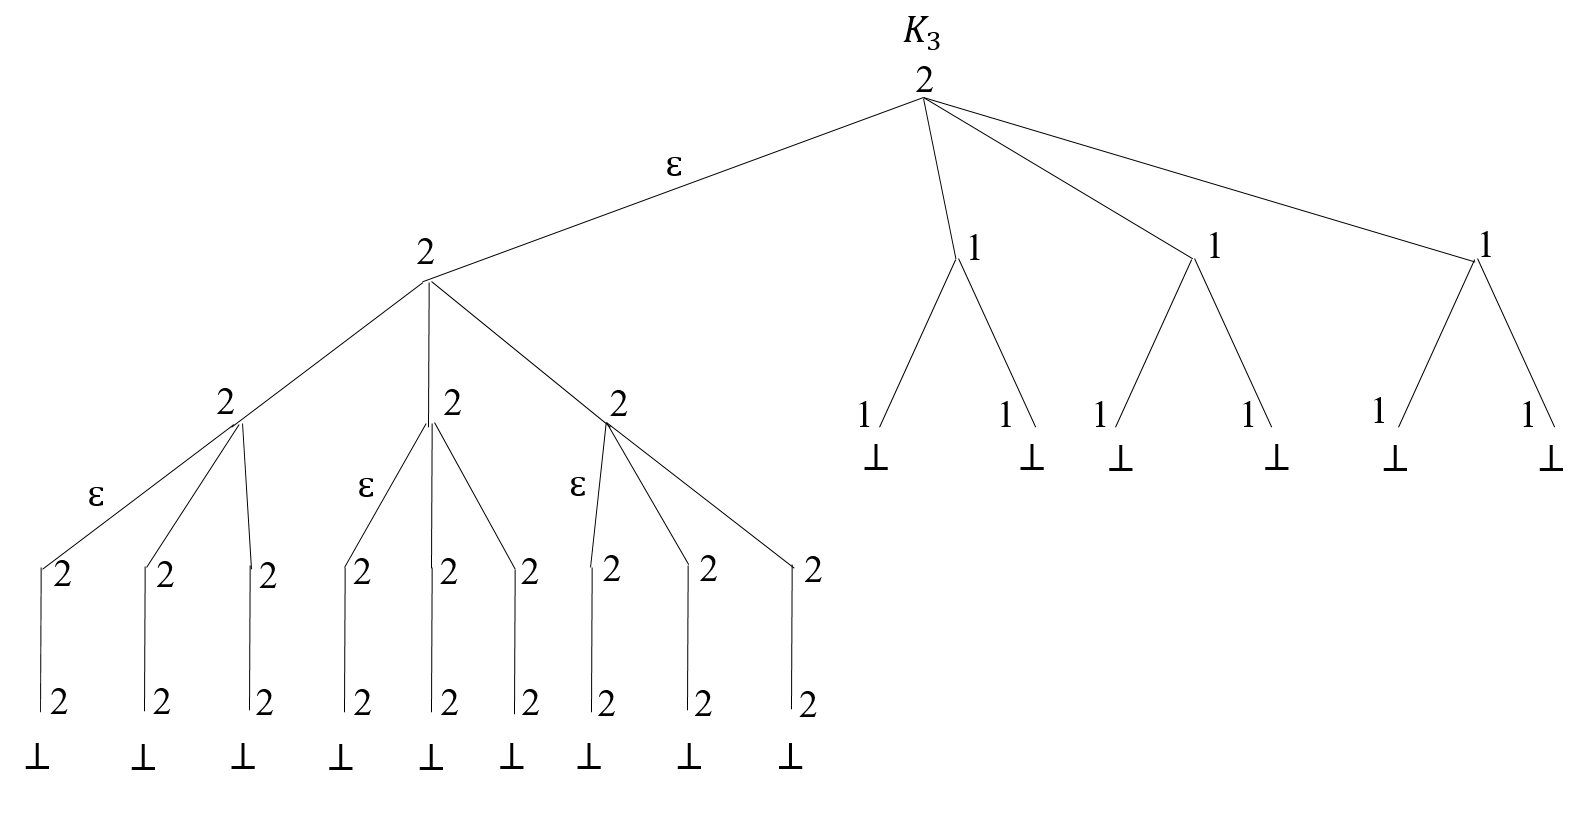
\includegraphics[scale =0.6]{gg1.png}
      \caption{??????? for $K_3$.}
	  \label{fig:gg1}
      \end{center}
      \end{figure}

\end{examp}  

%--------------------------------------------------------------------------------------------------------------------------------------
\section{The hardness game for Tseitin graph}
\label{sec:Hardness Tseitin}	  

In this section another measure to obtain hardness of a clause-set is presented in Lemma \ref{lem:game1} using hardness game according to \cite{h5}.

\begin{defi}\label{def:bridge}
      In graph theory, a \textbf{bridge} is an edge of a graph whose deletion increases its number of connected components. Equivalently, 
	  an edge is a bridge if and only if it is not contained in any cycle \cite{h15}.  
\end{defi}

\begin{lem}\label{lem:game1}
      Let $G$ be a Tseitin graph. Then $\hardness(X_0(G))$ is characterised by the following game:
	  \begin{enumerate}
	  \item An atomic move for the current non-trivial Tseitin graph $G$ replaces $G$ with a sub-graph $G'$ of $G$, obtained by choosing 
	  some $e \in E(G)$ and choosing a connected component of $G - e$.
	  \item The two players play in turns, and delayer starts with $G$.
	  \item A move of delayer is to apply a sequence of atomic moves (possibly zero).
	  \item A move of prover is to apply one atomic move.
	  \item The games ends when $G$ becomes trivial, in which case delayer gets as many points as there have been moves by prover.
	  \end{enumerate}
\end{lem} 
\begin{lem}\label{lem:game2}
      The hardness game has finitely many moves since the edges of a Tseitin graph are variables of $F$ based on Lemma \ref{lem:tgraph_2} and 
	  the number of variables in a clause-set is finite according to Definition \ref{def:cls}.
\end{lem}
\begin{lem}\label{lem:game3}
      The optimal value for hardness game of a graph would be in the case that both players play optimally. The optimal move for delayer 
	  is the one which maximises the hardness and the optimal move for prover is the one which minimises the hardness (or decreases $\hardness$ by one unit).
\end{lem}
\begin{lem}\label{lem:game6}
      If both player play optimally, there are two possible situations for prover; If there is no bridge in the graph then the optimal move for 
	  prover is not clear but based on Lemma \ref{lem:game1} it should remove an edge. If there is only one bridge, then according to lemma 
	  \ref{lem:game3}, the optimal move for prover is to remove the bridge and choose the smaller component. In both cases, the hardness is 
	  decreased by one unit. 
\end{lem}
\begin{lem}\label{lem:game4}
      Based on Lemma \ref{lem:game3}, we are not interested in prover plays optimally if delayer has already made a mistake.
\end{lem}


\begin{lem}\label{lem:game7}
      The optimal move for delayer if there is no bridge is to do nothing based on Lemma \ref{lem:game3}. If there is only one bridge 
	  which divides the graph into two componnents with $\hardness_1$ and $\hardness_2$, two cases may happen. If $\hardness_1= \hardness_2$, 
	  then it does not change the result whether delayer removes the bridge  and discards one of components or it chooses to do nothing and 
	  prover removes the bridge in next move and discards one of components (both moves are optimal). If $ \abs {\hardness_1- \hardness_2 } \geq 1$, 
	  then the optimal move is to remove the bridge and discard the smaller component based on Lemma \ref{lem:game3}. Finally, if there are 
	  more than one bridge in the graph, delayer removes all of them and chooses the component with biggest $\hardness$ and discards rest of 
	  components. If all components have the same hardness, delayer removes all bridges and keep one of components.
	  
\end{lem}

\begin{lem}\label{lem:game5}
      If prover can get two or more points by one move, then delayer has made a mistake before and based on Lemma \ref{lem:game4} the game can 
	  not be continued this way. The reason is that prover can get more than one point iff there is at least a bridge that divides the graph 
	  into two components with $ \abs {\hardness_1- \hardness_2 } > 1$ and according to Lemma \ref{lem:game7} delayer must already remove
	  all bridges and choose the component with biggest $\hardness$ and discard rest of components.
	  
\end{lem}
Remarks:
      \begin{enumerate}
	  \item According to previous lemmas, both delayer and prover have specific types of move which can be categorized (and named) as follows:
	       \begin{enumerate}
		   \item D-A: The graph has no bridge. So, according to Lemma \ref{lem:game7} delayer chooses to take no action.
		   \item D-B: There is only one bridge in graph. So, according to Lemma \ref{lem:game7} delayer removes the bridge and divides the graph 
		   into two components. Then, it chooses the bigger component and discards the smaller one.
		   \item D-C: (a move or conjecture????)If the graph has more than one bridge among $n$ components with different $\hardness$, based on 
		   Lemma \ref{lem:game7} delayer removes all of them and chooses the component with biggest $\hardness$ and discards rest of components.
		   %\item D-D: (In complete graphs) The graph is not symmetric but there is no bridge. If delayer removes any edge, 
		   %it might help prover to finish game earlier. Therefore, delayer prefers to take no action.		   
		   \item P-A: The graph has no bridge. So, according to Lemma \ref{lem:game6} prover must remove an edge.
		   %\item P-B: There is at least one node with one connected edge. Prover removes the edge and divides the graph into two components: 
		   %one isolated node and the rest of graph. Then, it chooses the isolated node and discards the rest of graph and the game finishes.
		   \item P-B: The graph has one bridge and according to Lemma \ref{lem:game6} prover removes the bridge and chooses the smaller component.
           \end{enumerate}		   
	  \item During the game, if we obtain a complete garph $K_n, n \in \NN$, the hardness would be the sum of prover's points (untill that step) 
	  and $\hardness(K_n).
	  \end{enumerate}

\begin{conj}\label{con:hd1}
     If there is a bridge in a Tseitin graph which connects two components with $\hardness_1$ and $\hardness_2$, then two cases may happen for 
	 $\hardness_{total}$. If $\hardness_1= \hardness_2$, then $\hardness_{total}= \hardness_1= \hardness_2$. Else, $ \abs {\hardness_1- \hardness_2 } \geq 1$
	 and if $ \hardness_1 > \hardness_2 $  then $\hardness_{total}= \hardness_1$.
	 
	 Explanation: Delayer starts the game and according to Lemma \ref{lem:game7} if $\hardness_1= \hardness_2$, then it does not change the result 
	 whether delayer removes the bridge or it chooses to do nothing and prover removes the bridge in next move. In both cases $\hardness_{total}$ 
	 would be equal to the hardness of the selected component. Otherwise, if $ \hardness_1 > \hardness_2 $ based on \ref{lem:game7} delayer 
	 removes the bridge and discards the smaller component. Untill now, prover has not done any thing and therefore, has not got any points.
	 In the next step, prover continues the game and  $\hardness_{total}= \hardness_1$.
\end{conj}

\begin{conj}\label{con:hd2}
           If the graph has no bridge and the number of connected edges to nodes are not equal then prover chooses the node with smallest
		   connected edges and removes one of them.
\end{conj}
	  
\begin{conj}\label{con:hd_game1}
      For a complete graph $K_n, n \in \NN$, $\hardness(K_n)= n-2+\hardness(K_{n-1})$. 
	  
	  Explanation: In a complete graph, there are $n-1$ connected edges to each node. Prover chooses a node and removes a connected edge of 
	  that node in each step. Then, when there is only one connected edge to that node(a bridge) delayer removes the bridge and chooses the 
	  $K_{n-1}$ graph. So, $\hardness(K_n)= (n-1)-1+\hardness(K_{n-1}) $.
	  Table \ref{fig:table1} showes $\hardness(K_n)$ for some $n$.
	  \begin{figure}[h]
       \centering
       \begin{tabular}{|c|c|} 
                  \hline
                  $n$ & $\hardness(K_n)$ \\ \hline
                 % 0 & 0  \\ \hline
                  %1 & 0  \\ \hline
				  2 & 1  \\ \hline
				  3 & $1+ \hardness(K_2)=2$ \\ \hline
			      4 & $2+ \hardness(K_3)=4$  \\ \hline
				  5 & $3+ \hardness(K_4)=7$  \\ \hline
				  6 & $4+ \hardness(K_5)=11$  \\ \hline
				  7 & $5+ \hardness(K_6)=16$  \\ \hline
       \end{tabular}
       \caption{The hardness for complete graph $K_n$.}
       \label{fig:table1}
      \end{figure}
\end{conj}

\begin{examp}\label{exp:hd1}
       Fig \ref{fig:game1} showes the atomic moves of hardness game for garph $K_3$ in Fig \ref{fig:hd1}. Delayer starts the game and two 
	   players play in turn. 
	   
	   In first move, the graph has no bridge and delayer chooses to do nothing. Then, prover chooses an edge (in this case, it can 
	   remove any edge). In third move, delayer has to do nothing since removing any edge will lead to ending game. Finally, prover 
	   chooses an edge and graph is divided to two components: one seprate vertex and one edge. So, prover chooses the vertex to 
	   finish the game. The hardness of the graph (which is the number of moves done by prover) is $\hardness(K_3)=2$.
	   
	   \begin{figure}[h]
       \centering
       \begin{tabular}{|c|c|} 
                  \hline
                  Delayer & Prover \\ \hline
                  nothing & choosing 1  \\ \hline
                  nothing & choosing 3  \\ \hline
       \end{tabular}
       \caption{The atomic moves for \ref{fig:hd1} and $\hardness(K_3)=2$.}
       \label{fig:game1}
      \end{figure}
	   %----------------------
	  \begin{figure}
      \begin{center}
	  %\centering
      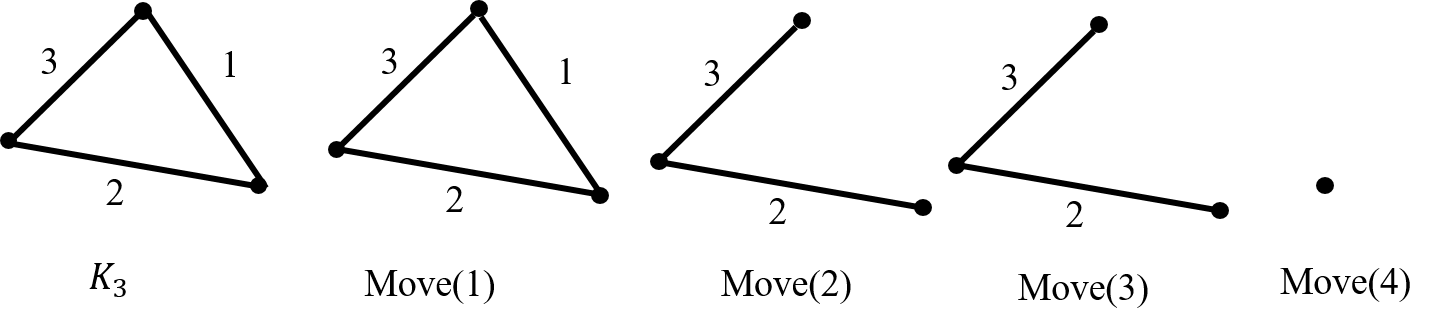
\includegraphics[scale =0.6]{g1.png}
      \caption{The hardness game for $K_3$.}
	  \label{fig:hd1}
      \end{center}
      \end{figure}
\end{examp}

\begin{examp}\label{exp:hd2}
       Fig \ref{fig:game2} showes the atomic moves of hardness game for garph $K_4$ in Fig \ref{fig:hd2}. Delayer starts the game and two 
	   players play in turn. 
	   
	   In first move, the graph has no bridge and delayer chooses to do nothing. Then, prover chooses an edge (in this case, it can remove any edge). 
	   In third move, delayer chooses to do nothing since there is no bridge. Then, prover can choose edges 1 or 4 (in this case we continue with removing edge 1) since in each case 
	   the result will be the same. In fifth move, delayer has to remove edge 6 (the bridge) and the graph is devided to two components: 
	   one seprate vertex and the $K_3$ graph. Delayer chooses biger component ( $K_3$ graph) and the rest of the game would be the same as Example \ref{exp:hd1} and $\hardness(K_4)=4$.
	 
	 \begin{figure}[h]
      \centering
      \begin{tabular}{|c|c|} 
      \hline
                  Delayer & Prover \\ \hline
                  nothing & choosing 2  \\ \hline
                  nothing & choosing 1  \\ \hline
                  choosing 6 & choosing 5  \\ \hline
                  nothing & choosing 4 \\ \hline
      \end{tabular}
      \caption{The atomic moves for Fig \ref{fig:hd2} and  $\hardness(K_4)=4$.}
      \label{fig:game2}
      \end{figure}
	  %---
	  \begin{figure}
      \begin{center}
	  %\centering
      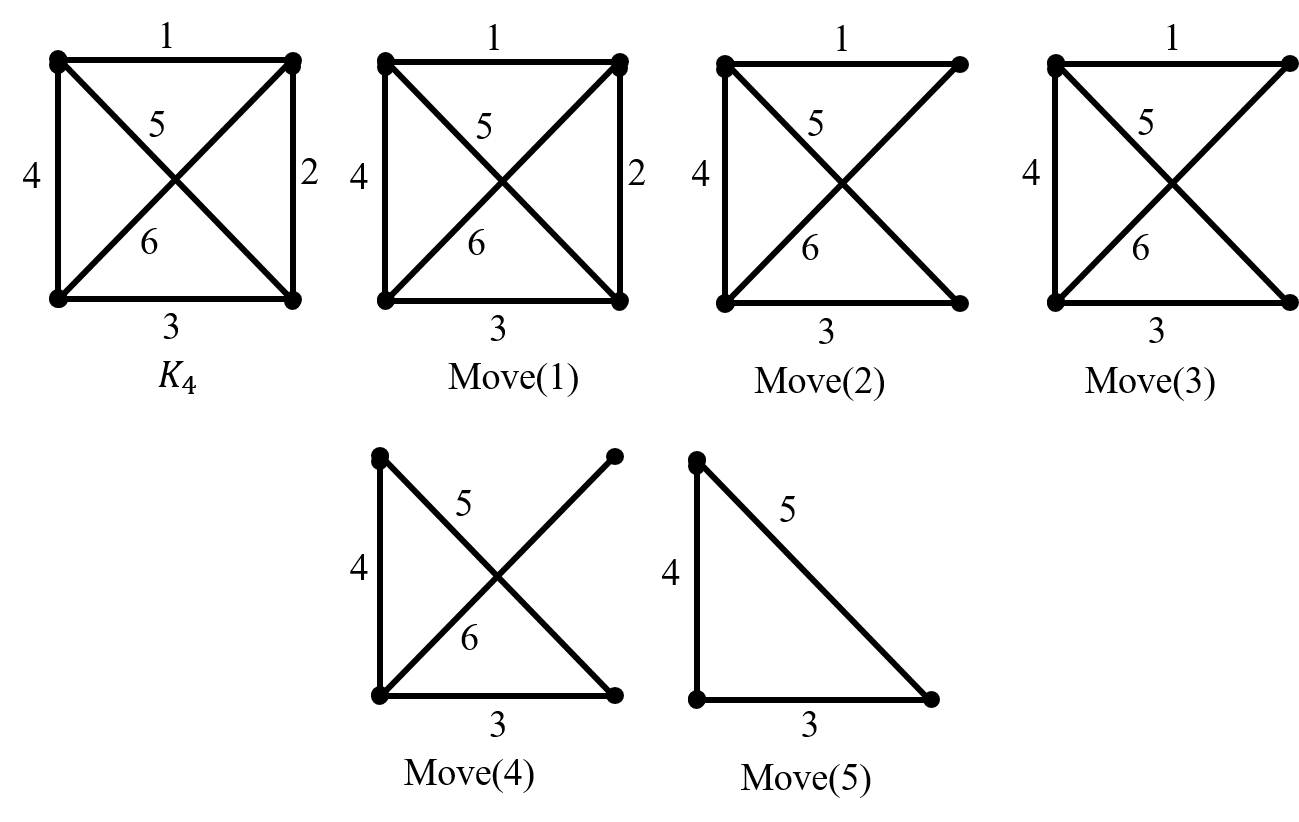
\includegraphics[scale =0.6]{g2.png}
      \caption{The hardness game for $K_4$}
	  \label{fig:hd2}
      \end{center}
      \end{figure}
	   
\end{examp}

\begin{examp}\label{exp:hd3}
       Fig \ref{fig:game3} showes the atomic moves of hardness game for garph $K_5$ in Fig \ref{fig:hd3}. Delayer starts the game and two 
	   players play in turn. 
	   
	   In first move, the graph has no bridge and delayer chooses to do nothing. Then, prover chooses an edge (in this case, it can remove 
	   any edge). In third move, delayer chooses to do nothing since there is no bridge. Then, prover chooses edge 5. Then, the delayer 
	   again chooses to do nothing since there is no bridge. In the next move, the prover chooses edge 10. Therefore delayer has to remove 
	   edge 7 (the bridge) and the graph is devided to two components: one seprate vertex and the $K_4$ graph. Delayer chooses biger component 
	   ($K_4$ graph) and the rest of the game would be the same as Example \ref{exp:hd2} and $\hardness(K_5)=7$.
	 
	   \begin{figure}[h]
      \centering
      \begin{tabular}{|c|c|} 
      \hline
                  Delayer & Prover \\ \hline
                  nothing & choosing 1  \\ \hline
				  nothing & choosing 5  \\ \hline
				  nothing & choosing 10  \\ \hline
                  choosing 7 & choosing 4  \\ \hline
				  Nothing & choosing 3  \\ \hline
                  choosing 8 & choosing 9  \\ \hline
				  nothing & choosing 2  \\ \hline
      \end{tabular}
      \caption{The atomic moves for Fig \ref{fig:hd3} and \hardness(K_5)=7.}
      \label{fig:game3}
      \end{figure}
	   %-----------------
	  \begin{figure}
      \begin{center}
	  %\centering
      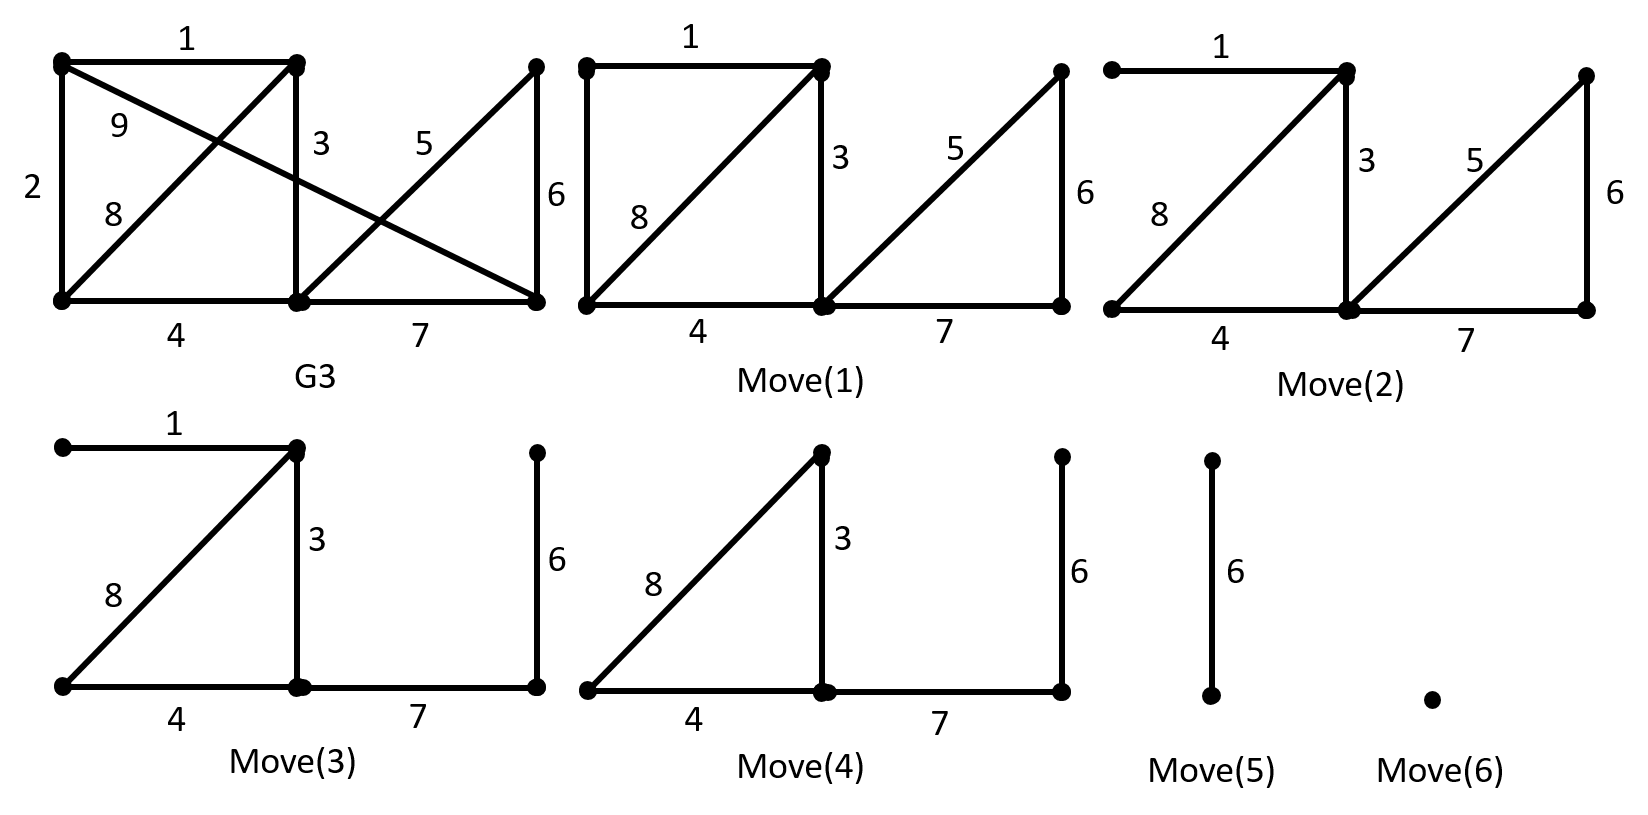
\includegraphics[scale =0.6]{g3.png}
      \caption{The hardness game for $K_5$}
	  \label{fig:hd3}
      \end{center}
      \end{figure}
\end{examp}

\begin{examp}\label{exp:hd4}
       Fig \ref{fig:game4} showes the atomic moves of hardness game for garph $G_1$ in Fig \ref{fig:hd4}. Delayer starts the game and two 
	   players play in turn. 
	   
	   In first move, the graph has no bridge and delayer chooses to do nothing. Then, prover chooses a vertex with the least number of 
	   connected edges and removes one of edges (edge 5). In next move, delayer finds a bridge (edge 6) and removes it and discards the 
	   smaller component (the isolated vertex). Then, prover chooses another vertex with the least number of connected edges and removes 
	   one of edges (edge 9). Delayer, again, finds a bridge (edge 7) and removes it. After that, prover removes edge 3 and in next move, 
	   delayer removes the bridge (edge 4). In this step, the left component is graph $K_3$ and the rest of game is the same as Example 
	   \ref{exp:hd1}. So, $\hardness(G_1)=3+\hardness(K_3)=5$.
	 
	   \begin{figure}[h]
       \centering
       \begin{tabular}{|c|c|} 
       \hline
                  Delayer & Prover \\ \hline
                  nothing & choosing 5  \\ \hline
				  choosing 6 & choosing 9  \\ \hline
				  choosing 7 & choosing 3  \\ \hline
				  choosing 4 & choosing 8  \\ \hline
				  nothing & choosing 2  \\ \hline

      \end{tabular}
      \caption{The atomic moves for Fig \ref{fig:hd4}.}
      \label{fig:game4}
      \end{figure}
	   %-----------------
	  \begin{figure}
      \begin{center}
	  %\centering
      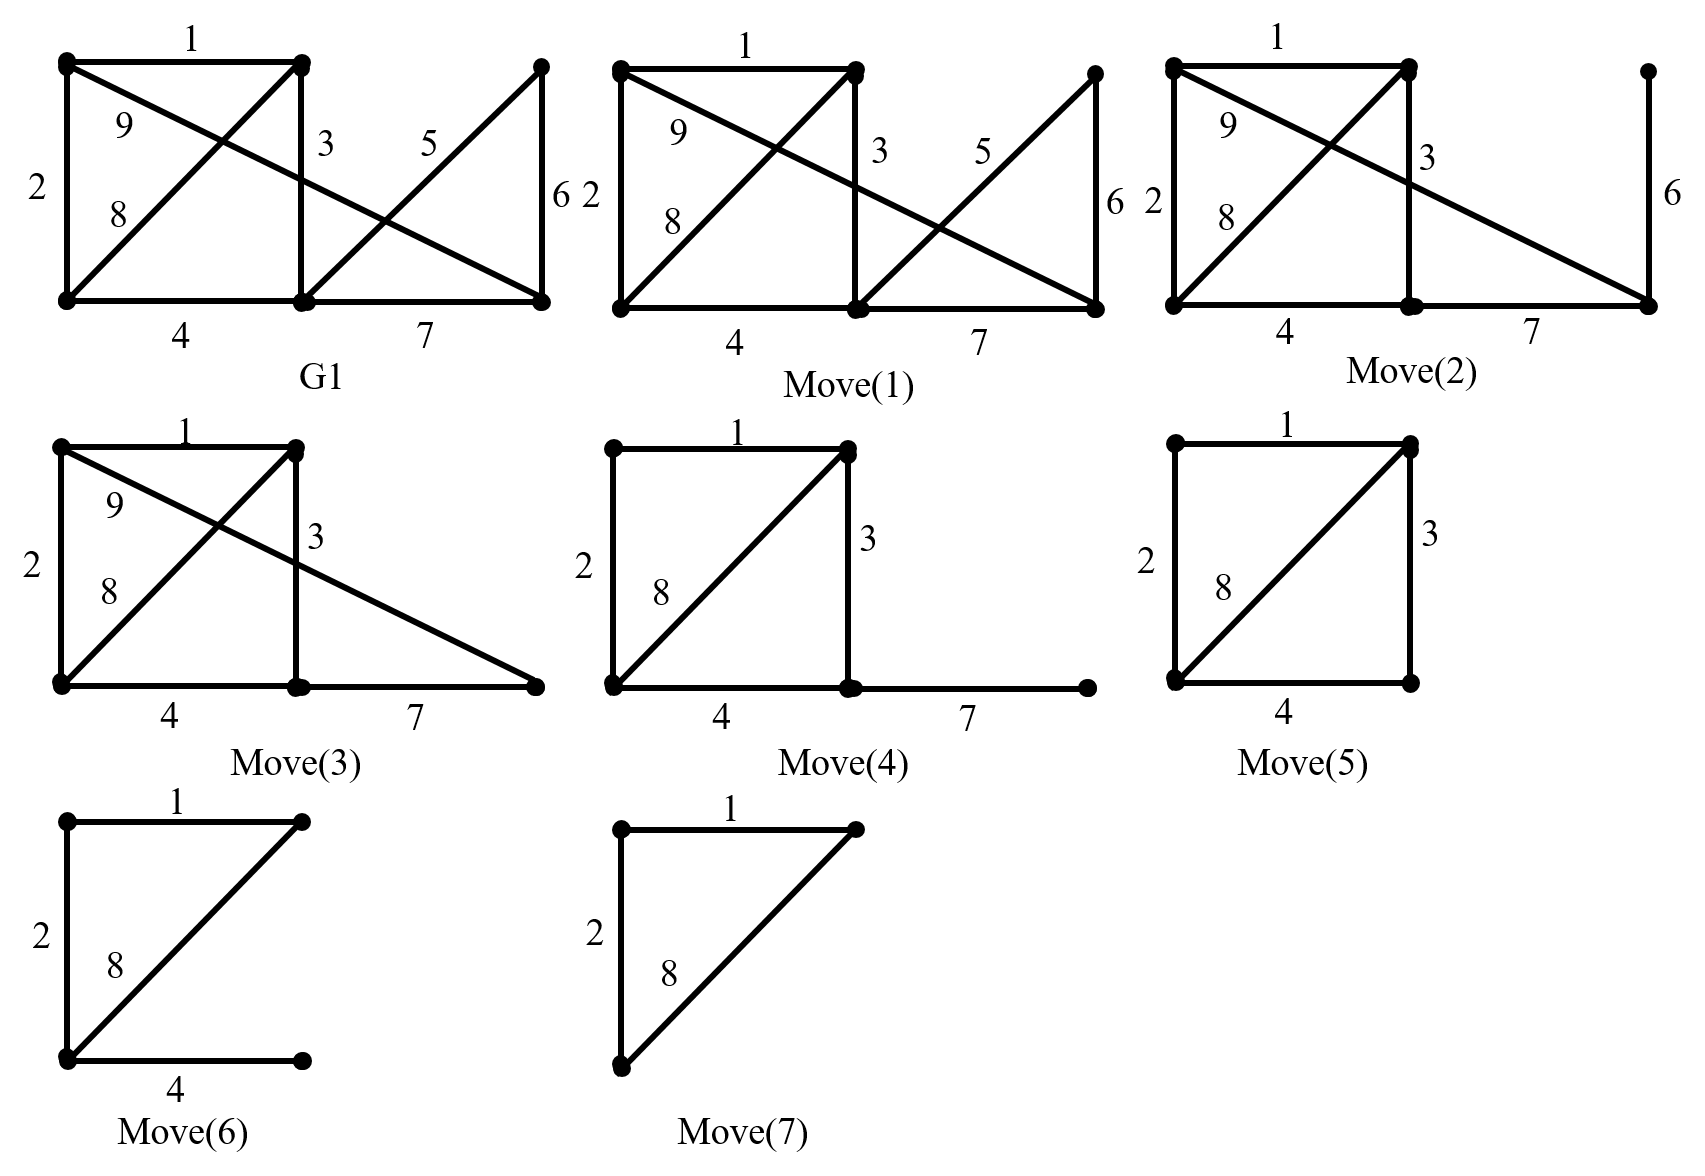
\includegraphics[scale =0.57]{graph_hd1.png}
      \caption{The hardness game for  $G_1$}
	  \label{fig:hd4}
      \end{center}
      \end{figure}
\end{examp}

\begin{conj}\label{con:hd_game2}
     If a Tseitin graph does not have any parallel edges then for $n$ vertices, graph $K_n$ has the worst case of hardness 
	 (the maximum of $\hardness$) which is equal to $\hardness(K_n)= n-2+\hardness(K_{n-1})$ according to Conjecture  \ref{con:hd_game1}.
	 
	 Explanation:???????????
\end{conj}

\begin{conj}\label{con:hd_game3}
           Consider a graph that has more than a bridge among $n$ components with different $\hardness$. If we assume that 
		   the hardness of each component is known, then delayer should remove all of bridges and keep the component with 
		   biggest hardness.
		   
		   Explanation: We know from Lemma \ref{lem:game3} that delayer tends to maximise $\hardness$ which means it want to prolong
		   the game. If we suppose that delayer does not remove all bridges in first move, there will be at least a bridge which 
		   connects two components with different $\hardness$ in the next move. So, prover will remove the bridge and choose the
		   component with smaller $\hardness$. If $ \abs {\hardness_1- \hardness_2 } > 1$, prover gets more than one point in one move
		   which according to Lemma \ref{lem:game5} showes that delayer has made a mistake. If $\hardness_1- \hardness_2  = 1$, then
		   prover gets one point by removing the bridge and discarding the bigger component. So, the result might be correct but 
		   delayer might already discard the biggest component. In that case, prover might get more points during the game which leads 
		   to bigger $\hardness$! Therefore, delayer has not played optimally.
		   
		   ???????????		   
\end{conj}

\begin{examp}\label{exp:hd5}
       Fig \ref{fig:hd5} showes an example of a graph with 6 components (whose $\hardness$ is known) and 5 bridges. In first move,
	   according to Conjecture \ref{con:hd_game3} delayer should remove all bridges and keep component 1. Otherwise, if any bridges is 
	   left prover will remove the bridge and choose the smaller component and $\hardness$ will not be the optimal value.
	   Therefore, total $\hardness$ for $G_2$ is equal to the $\hardness$ of component 1.	   

	   %-----------------
	  \begin{figure}
      \begin{center}
	  %\centering
      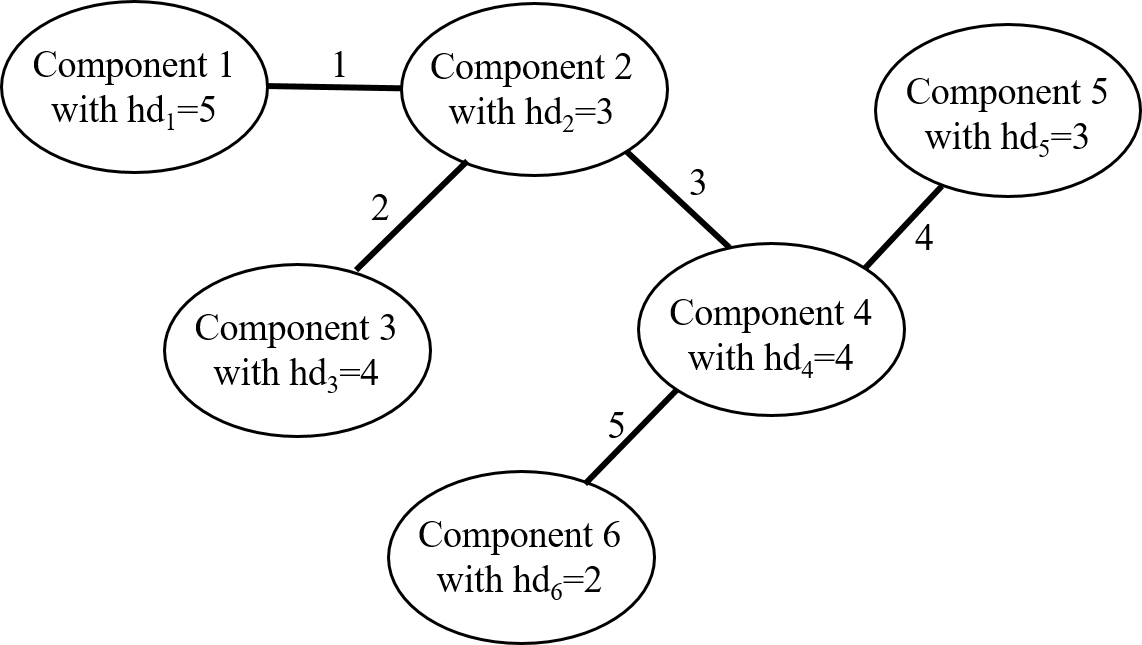
\includegraphics[scale =0.65]{graph_with_bridges.png}
      \caption{Graph $G_2$ with 5 bridges}
	  \label{fig:hd5}
      \end{center}
      \end{figure}
\end{examp}

\begin{examp}\label{exp:hd6}
       Consider Fig \ref{fig:hd6}, a graph with two components 1 and 2 with $\hardness=5$ which have biggest hardness compared
	   to other components. In this case if delayer removes all bridges and keeps one of components 1 or 2, the total $\hardness$ 
	   would be 5. But, if delayer removes all bridges except bridge 1, then prover will continue by removing bridge 1 and discarding 
	   one of components (and getting one point). In this case, total $\hardness$ will be 5+1. So, based on Lemma \ref{lem:game3}, 
	   delayer keeps bridge 1 in the first move and total $\hardness$ is 6.
	   %-----------------
	  \begin{figure}
      \begin{center}
	  %\centering
      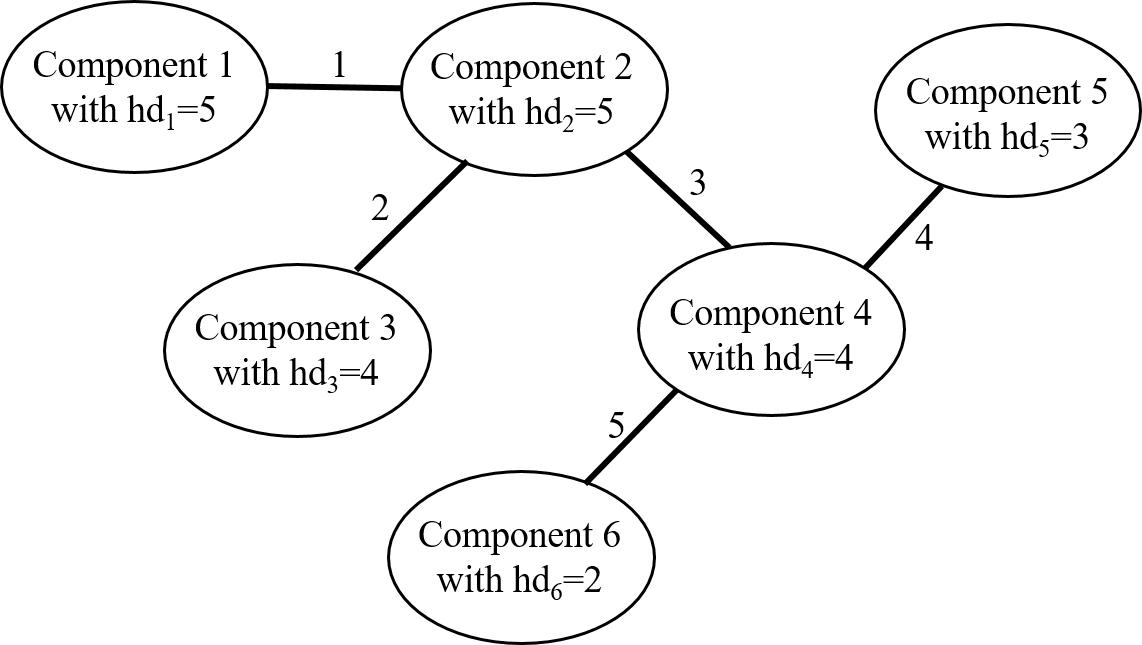
\includegraphics[scale =0.65]{graph_with_bridges2.png}
      \caption{Graph $G_3$ with 5 bridges}
	  \label{fig:hd6}
      \end{center}
      \end{figure}
\end{examp}


%***************************************************************************************************************************************
%***************************************************************************************************************************************************************
\chapter{Conclusion and open problems}
\label{cha:concl}

\section{Questions}
\label{sec:Questions}

\begin{quest}\label{que:q1}
      Is there any relation among various hardness measures?
\end{quest}

\section{Conclusion}
\label{sec:Conclusion}
%--------------------------------------------------------------------------------------------------------------------------------------

%--------------------------------------------------------------------------------------------------------------------------------------
\newpage
\bibliography{HA_ResearchRef}
\bibliographystyle{plainurl}


\end{document}

